% main_apsec.tex: APSEC 2026 SEIP paper (<=10 pages incl. appendix + 1 page of refs).
% Scope: the tool IN PRACTICE, evidenced by a two-condition user study.
% The scoring-policy analysis, the verdict-sensitivity bound, the multi-model
% study and the decision study with decision makers belong to a separate
% research paper and must not appear here.
\documentclass[10pt,conference]{IEEEtran}
\IEEEoverridecommandlockouts

\usepackage{cite}
\usepackage{amsmath,amssymb,amsfonts}
\usepackage{graphicx}
\usepackage{booktabs}
\usepackage{tabularx}
\usepackage{array}
\usepackage{microtype}
\usepackage{siunitx}
\usepackage{xcolor}
\usepackage{hyperref}
\usepackage{cleveref}
\usepackage{etc}
\definecolor{brandgreen}{HTML}{00915A}
\hypersetup{colorlinks=true,allcolors=brandgreen}
\newcommand{\best}[1]{\textbf{#1}}
\newcommand{\cmark}{\textcolor{brandgreen}{\textbf{Y}}}
\newcommand{\xmark}{\textcolor{black!35}{--}}

\newcolumntype{L}[1]{>{\raggedright\arraybackslash}p{#1}}
\newcommand{\tblsetup}{%
  \footnotesize%
  \setlength{\tabcolsep}{3pt}%
  \renewcommand{\arraystretch}{1.02}%
}

% At most one full-width float at the top of a page: two stacked diagrams
% leave no readable text behind them.
\setcounter{dbltopnumber}{1}

% Tighter float spacing than the IEEEtran defaults (page budget).
\setlength{\textfloatsep}{7pt plus 2pt minus 3pt}
\setlength{\dbltextfloatsep}{7pt plus 2pt minus 3pt}
\setlength{\floatsep}{7pt plus 2pt minus 2pt}
\setlength{\dblfloatsep}{7pt plus 2pt minus 2pt}
\setlength{\abovecaptionskip}{4pt}

% !! Flip to true once data/user_study/{quiz,survey}.csv are collected and
% scripts/analyze_user_study.py --quiz has produced the numbers. The \else
% branch keeps the paper compiling with visible placeholders in the meantime.
\newif\ifstudydone
\studydonetrue
% Filled from `make study-export` output when the flag above is flipped.
\newcommand{\studyN}{eight}
\newcommand{\studyCell}{\textit{--}}
\providecommand{\repourl}{https://github.com/Rqbln/VERA}

\begin{document}

\title{VERA: An Operable Dashboard for Assessing\\ LLM Deployments in Light of the EU AI Act}

% APSEC SEIP is not double-anonymous, so this paper always builds named. The
% block lives in authors_apsec.tex, which is NOT version-controlled: the
% anonymized mirror proxies this repo, so tracked sources carry no identity.
% It is deliberately separate from authors.tex, which serves main.tex (ICSE):
% the two papers do not share an author list.
\author{%
  \InputIfFileExists{authors_apsec}{}{%
    \IEEEauthorblockN{Author list withheld}
    \IEEEauthorblockA{authors\_apsec.tex is absent from this checkout}%
  }%
}

\maketitle

\begin{abstract}
Institutions that deploy large language models in regulated settings must document technical evidence across the six principles the EU AI Act sets out, including environmental impact, before a deployment is approved.
The suites that produce this evidence run from a command line, while the staff who approve deployments work in compliance and risk management and do not write code.
The evidence therefore arrives through an engineer, summarised into a slide and stripped of the detail a reviewer needs to question it.
We present VERA, an open-source self-hosted platform in production in the responsible-AI function of a large European bank.
A reviewer selects a model, runs public benchmarks against it, and reads one score per regulatory requirement, where each score opens onto the tests behind it and each export names the run it came from.
VERA scores the twelve requirements that current benchmarks can measure and adds a thirteenth by instrumenting the energy each evaluation consumes, so environmental impact becomes a measured verdict rather than a written attestation.
Six open-weight models across three families and three sizes exercise all thirteen, and a within-subject study administered by the platform then measures what the presentation changes for a reader.
Across eight participants, correct answers rise from 18 to 32 of 48 and the median time per question falls from 56 to 29 seconds.
The condition order is fixed and the participants are research staff rather than compliance reviewers, so we report an effect on reading rather than on decisions.
VERA and the study instrument are released, so any institution under the same obligation can repeat the measurement on its own deployment, and so the people accountable for an AI release can work from evidence rather than from assurances.
\end{abstract}

\begin{IEEEkeywords}
Responsible AI, EU AI Act, Compliance tooling, User study, Software engineering in practice, Open source
\end{IEEEkeywords}

\section{Introduction}
\label{sec:intro}

Large language models are being built into products across almost every customer-facing function, from answering queries to triaging support requests and drafting documents.
These models are non-deterministic, since their behaviour is learned from the data they are trained on rather than specified by rules, so the same input can produce different outputs across runs.
The same property also leads models to generate confident but false statements, known as hallucinations~\cite{lin2022truthfulqa}, to reproduce text from their training data~\cite{carlini2023extracting}, and to answer the same question differently depending on the social group it names, such as a gender, an ethnicity or a religion~\cite{parrish2022bbq}.
Conventional testing cannot catch behaviour of this kind, since there is no single expected output against which a response can be checked.
Practitioners therefore measure it statistically, over benchmark suites that probe each failure mode~\cite{hendrycks2021mmlu,gehman2020realtoxicity}.

The severity of these failures has led regulators to require such measurement by law rather than leave it to good practice.
The EU AI Act is the most far-reaching of these regulations, and it obliges the provider of a high-risk system to document technical evidence that the system meets a defined set of requirements before it can be deployed~\cite{euaiact2024}.
That evidence must cover the six principles the Act sets out in Recital~27, namely human agency and oversight, technical robustness and safety, privacy and data governance, transparency, diversity and fairness, and social and environmental well-being~\cite{euaiact2024,hleg2019trustworthyai}.
This makes evidence production a routine engineering task that every deployment must complete before it proceeds.

\begin{figure*}[t]
  \centering
  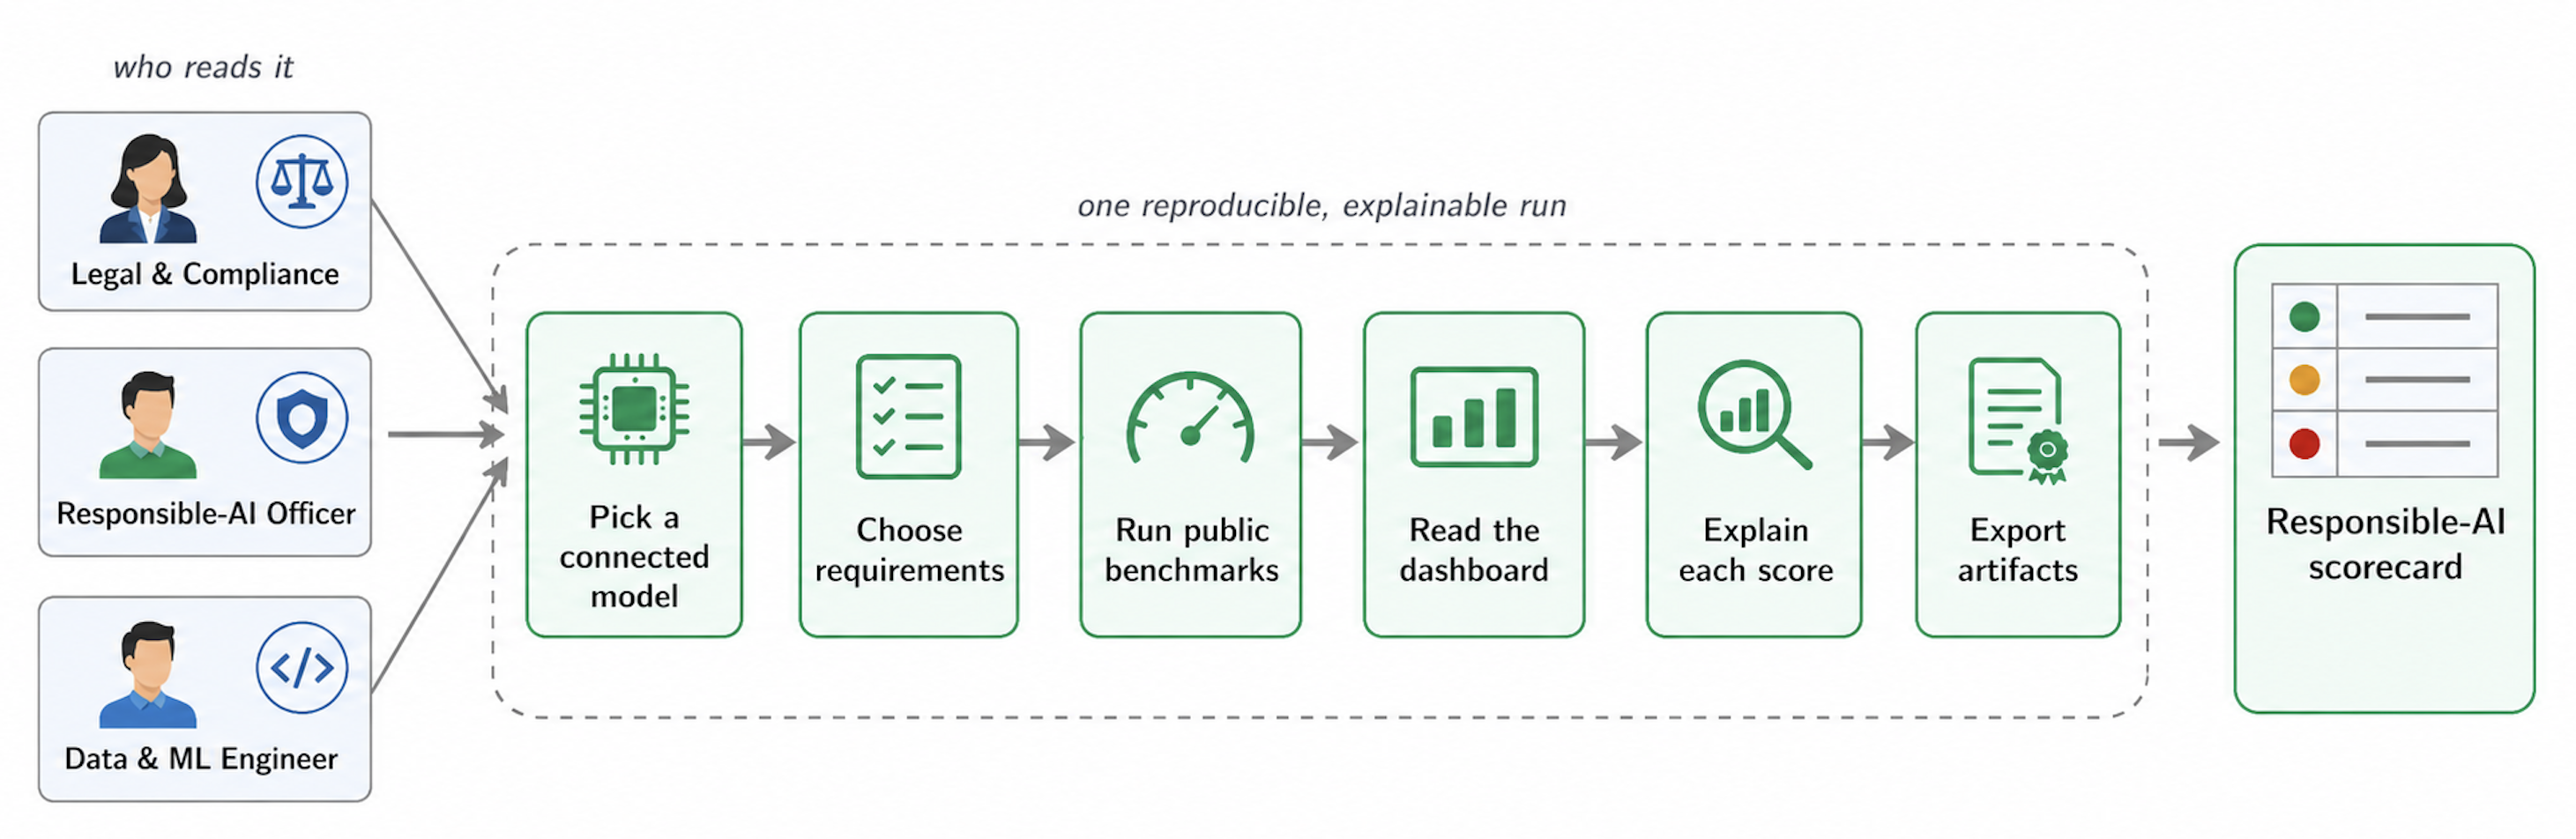
\includegraphics[width=0.80\textwidth]{figures/fig1}
  \caption{The path a user follows, whatever the role. The user selects a served model and a requirement set, runs public benchmarks against it, reads the outcome through a view filtered to that role in which each score can be opened, and exports the evidence tied to that run. 
  % \todo{have we referenced it somewhere?} 
  }
  \label{fig:journey}
\end{figure*}

In a regulated institution, however, the people who produce this evidence and the people accountable for the deployment are not the same.
Approval rests with the second line of defence, in compliance or in risk management, while the evaluation suites are operated by engineers.
Over a year of preparing release decisions in the responsible-AI function of BNP Paribas, we observed three problems that recur because of this separation.
The first is access, since every suite is driven from a command line.
An engineer therefore runs the evaluation and brings a summary slide to the review meeting, where the reviewers cannot interrogate the numbers on it.
The second is opacity, since results arrive as a table of scores with no link to the tests behind them.
A reviewer who asks why a requirement scored poorly must match the run record against per-item outputs by hand.
In one review, a reviewer asked which benchmarks had produced an artificial-intelligence disclosure score of $0.50$ for one model, and answering meant scanning a 209-line harness log to isolate the ten self-disclosure responses behind that requirement, even though every fact needed was already in the files.
The third is drift.
Release documentation is written after the run, so by the time it is filed it describes an evaluation that has already changed.
All three are properties of the software that delivers the measurements rather than of the measurements themselves.

The measurement itself is already well supported.
COMPL-AI maps the Act's principles to eighteen technical requirements and connects twelve of them to public benchmarks~\cite{guldimann2024complai}, while the suites beneath it fix which scenarios a report covers and how each benchmark is executed~\cite{liang2023helm,gao2021lmevalharness,derczynski2024garak,wang2023decodingtrust}.
Run against a served model, these tools write a run record, a harness log and the per-item outputs, which together hold every fact a reviewer needs.
None of them, however, supports reading those files.
Opening them requires a command line, nothing links a requirement score back to the tests that produced it, and the documentation a reviewer takes away does not record which run it came from.
Access, opacity and drift therefore survive a complete measurement, and closing them is the first gap this work addresses.
A second gap lies inside the taxonomy itself, since the remaining six are written up rather than measured, and environmental impact is one of them.
It differs from the other five, because corrigibility and explainability have no agreed technical definition, whereas energy draw is a physical quantity that the Act asks providers to document (Art.~40 Para~2, Annex~XI Para~2e)~\cite{euaiact2024}.
COMPL-AI collects that figure through a form about the resources used in training, although the energy an evaluation itself consumes can be read directly from the host that runs it~\cite{rajput2024fecom}.

To close both gaps, we built VERA (Verifiable Evaluation for Responsible AI), a self-hosted platform that enables a non-specialist to run a requirement-based evaluation of a served model and to read the evidence it produces, from the launch of the run to the filed artifact, and put it into production in the responsible-AI function described above.
A reviewer selects a served model, runs the public benchmark suites against it, and reads a score for each regulatory requirement.
Any score opens onto the benchmarks that produced it and the answers the model gave.
The export that leaves the review names the run behind it, so a later reader can check a figure rather than trust it.
VERA scores all twelve requirements the reference taxonomy can measure, and it adds a thirteenth by instrumenting the energy each evaluation consumes, so environmental impact becomes a measured verdict rather than a written attestation.
Five of the eighteen then remain on a documented human path, rather than six.
\Cref{fig:journey} shows the route a reviewer takes, which needs no account, no configuration file and no code.
A reading layer has to produce output at all before its presentation can matter, so we evaluate VERA on both.
We first run all twelve measurable requirements over six open-weight models, three families at a comparable size and one family at three sizes, which shows that the tool executes the full taxonomy and separates the models it scores.
We then run a within-subject study administered by the platform itself, in which each of eight participants answers six factual questions about one completed evaluation from its raw files and six matched questions on VERA, while the application times each question and validates each answer.
The condition order is fixed and the participants are research staff rather than the compliance reviewers the tool targets, so we report the comparison as an effect on reading rather than on decisions.

This paper makes the following contributions.


\begin{enumerate}
   \item We present VERA, an open-source self-hosted platform that turns a completed evaluation into requirement verdicts a reviewer can read, expand to the tests and model responses behind them, and export with the identity of the run that produced them.
  \item We extend the measurable requirement set from twelve to thirteen by instrumenting the energy each evaluation run consumes, so environmental impact becomes a measured verdict rather than a written attestation.
  \item We provide controlled evidence that presenting an evaluation per regulatory requirement improves the facts a reviewer extracts from it, using a within-subject study that the platform administers.
  \item We identify where that presentation fails, since aggregating benchmarks per requirement hides the coverage a reviewer must count, and a guided launch path does not by itself make a run reachable.
  \item We release the platform, the study instrument that produced these measurements, and the analysis script, available at \url{\repourl}.
\end{enumerate}

% VERA and the study module are available at \url{\repourl}.

% \todo{you dont need this in a 10 page paper.}
% The remainder of this paper is organised as follows.
% \Cref{sec:background} reviews the work on measuring and on reading an evaluation, and states the six requirements.
% \Cref{sec:vera} describes VERA, its six features and its energy instrumentation.
% \Cref{sec:study} gives the evaluation design and \Cref{sec:results} the results.
% \Cref{sec:discussion} interprets those results, \Cref{sec:threats} states what bounds them, \Cref{sec:lessons} reports the deployment experience, and \Cref{sec:conclusion} concludes.

\section{Background and Related Work}
\label{sec:background}

Measuring a model and reading that measurement are separate problems, and the literature has solved only the first.
This section reviews the work on each.

\subsection{Benchmark Suites and Requirement Taxonomies}
COMPL-AI is an independent effort by ETH Zurich, INSAIT and LatticeFlow AI that maps the Act's principles to eighteen technical requirements and connects twelve of them to public benchmarks~\cite{guldimann2024complai}.
It is neither funded by the European Union nor part of the Act's harmonised standards, and it publishes a study and a public leaderboard rather than a tool an operator can drive.
The taxonomy it defines is therefore available to a practitioner, while the means of operating it is not.

The suites beneath that taxonomy execute the tests.
HELM fixes which scenarios a report covers~\cite{liang2023helm}, the language model evaluation harness fixes how a benchmark runs so that two runs are comparable~\cite{gao2021lmevalharness}, Garak probes for jailbreaks~\cite{derczynski2024garak}, and DecodingTrust bundles a trustworthiness suite~\cite{wang2023decodingtrust}.
Each answers a measurement question in isolation, and none reports its result against a regulatory requirement.
A separate line of research applies natural-language processing to the regulation itself, extracting obligations from legal text and checking artifacts against them~\cite{abualhaija2025llmregextraction,amaral2022nlpcompliance,abualhaija2024regchange}.
Deriving a requirement set is a different problem from operating one that already exists, and this paper addresses the second.

\subsection{Tool Support for Reviewing Results}
Running these suites against a served model yields a run record, a harness log and the per-item outputs, and \Cref{tab:related} compares what a reviewer can then do with that output.
The table shows a complete measurement layer above an absent reading layer.
Only COMPL-AI reports at the requirement level, none offers an interface that a non-specialist can use, and opening a score to see the tests behind it is at best partial.
No suite provides role-filtered views or run-tied artifacts, and both omissions have practical consequences.
A legal reviewer and a data scientist are accountable for different subsets of the same evidence, and an export that does not name its run cannot be filed against Annex~IV.

The layers around the suites leave the same need unmet.
The NIST and ISO frameworks guide organisational risk management without prescribing runnable metrics~\cite{nist2023airmf,iso42001_2023}.
Model Cards and Datasheets standardise what a description of a model or a dataset should say, and both are authored rather than generated, since a writer produces them after the run they describe~\cite{mitchell2019modelcard,gebru2021datasheets}, which is the drift identified in \Cref{sec:intro}.
PromptOps is the closest work on the reading side and identifies the same interface problem, although it scores prompt by prompt and reports a flat set of numbers rather than a verdict a reviewer can expand~\cite{sunetnanta2025promptops}.

One requirement is missing from the measurement layer as well as from the reading layer.
None of these tools reports the energy its own evaluation consumes, so environmental impact stays a requirement a provider describes rather than measures.
Techniques for measuring that quantity already exist in software engineering research.
In our prior work we measured the energy of deep-learning code at method and interface granularity, and we showed that coarse attribution misstates where energy is spent~\cite{rajput2024fecom,rajput2024greenlight}.
More recent work reports the energy cost of running large language models on standard benchmarks~\cite{mehditabar2025smart}.
Neither line has yet been connected to the reporting obligation.

\begin{table*}[t]
  \caption{What a reviewer can do with each tool's output. \cmark{} = provided, \xmark{} = absent, Partial = present but incomplete.}
  \label{tab:related}
  \centering
  \tblsetup
  \begin{tabularx}{\textwidth}{@{}l*{7}{>{\centering\arraybackslash}X}@{}}
    \toprule
    Tool & Requirement view & Non-specialist UI & Decomposable verdicts & Role-based views & Run-tied artifacts & Swappable specification & Energy measured per run \\
    \midrule
    COMPL-AI~\cite{guldimann2024complai} & \cmark & \xmark & Partial & \xmark & \xmark & Partial & \xmark \\
    HELM~\cite{liang2023helm} & \xmark & \xmark & Partial & \xmark & \xmark & Partial & \xmark \\
    lm-evaluation~\cite{gao2021lmevalharness} & \xmark & \xmark & \xmark & \xmark & \xmark & \cmark & \xmark \\
    Garak~\cite{derczynski2024garak} & \xmark & \xmark & \xmark & \xmark & \xmark & \cmark & \xmark \\
    DecodingTrust~\cite{wang2023decodingtrust} & Partial & \xmark & Partial & \xmark & \xmark & \xmark & \xmark \\
    PromptOps~\cite{sunetnanta2025promptops} & \xmark & \cmark & Partial & \xmark & \xmark & \xmark & \xmark \\
    VERA (this paper) & \cmark & \cmark & \cmark & \cmark & \cmark & \cmark & \cmark \\
    \bottomrule
  \end{tabularx}
  \\[2pt]
  {\footnotesize \emph{Requirement view}: results reported per regulatory requirement rather than per prompt or scenario. \emph{Decomposable verdicts}: a verdict opens, inside the tool, down to the benchmarks behind it. \emph{Run-tied artifacts}: documentation emitted by the run rather than authored afterwards. \emph{Energy measured per run}: the tool reports the energy its own evaluation consumed, which none of the existing tools does. Each existing tool was assessed against its public documentation and source, and the VERA row states the properties \Cref{sec:vera} describes. \todo{Record the version and access date per row, since a reviewer who checks one row against a newer release will discount the table.}}
\end{table*}

\section{The VERA Platform}
\label{sec:vera}
\todo{refer: \label{fig:journey}}
VERA presents a completed evaluation as a set of requirement verdicts that a reviewer can read, expand and export in a browser, and it derives those verdicts from public benchmark suites rather than from measurements of its own.
It adopts the COMPL-AI taxonomy without modification, so its requirement identifiers and score ranges match the published reference, and it is implemented as a Python~3.11 backend with a TypeScript single-page front end.
This section states the six requirements the design answers, follows a request through the backend, describes the six features, and closes with the energy instrumentation behind the environmental-impact verdict.

\subsection{Requirements from Practice}
\label{sec:requirements}
\Cref{tab:related} identifies what the available tools omit in general, while release reviews conducted under internal-control obligations show which of those omissions matter in a deployment.
The six requirements record the authors' experience of preparing release decisions across a year. We followed no systematic elicitation protocol, and we state the source of each requirement so that a reader can weigh it accordingly\todo{we need to add refs for each with some justification}.
We state the source of each requirement, since the source determines how far it generalises beyond the setting it comes from.

\textbf{R1, from observed practice.}
A non-specialist must be able to run an evaluation and read its verdict without writing code, which restates the access failure of \Cref{sec:intro} as a requirement.
PromptOps reaches the same conclusion for developers~\cite{sunetnanta2025promptops}.

\textbf{R2, from practice and the literature.}
Every verdict must expand to the public tests that produced it, since a single aggregate hides why a model fails and leaves a reviewer with nothing to question.

\textbf{R3, from regulatory text and the design decision it motivates.}
The Act fixes what the technical file of a high-risk system must contain (Art.~11, Annex~IV) without prescribing how that file is produced.
We therefore add a production constraint of our own and require every piece of evidence to carry the identity of the run it came from, since documentation written afterwards describes an evaluation that has already changed.

\textbf{R4, from observed practice.}
Views must differ by role, since legal, responsible-AI and data-science reviewers are accountable for different subsets of the evidence and describe them in different vocabulary.

\textbf{R5, from observed practice.}
The requirement set and the benchmarks must be replaceable without a code change, because our first version hard-coded the taxonomy and every disputed weight then cost a release.

\textbf{R6, from institutional constraint.}
The tool must be self-hostable with no proprietary cloud dependency, since prompts and outputs cannot transit through a third party.

\subsection{Architecture}
\Cref{fig:architecture} follows a launch request until it becomes a scored and documented run.
Three surfaces can issue that request, namely a command line, a REST endpoint and a guided wizard that needs no login, and all three normalise it into one declarative job on a Celery and Redis queue.
A single job description behind three entry points makes a wizard run and a command-line run produce the same artifacts, so a non-specialist and an engineer read identical evidence.
A worker then resolves each requirement to its benchmarks through a registry, drives the runners against self-hosted models through a local router, and folds the cached item scores into per-requirement scores with bootstrap intervals.
The worker emits a bundle holding the run file, the model card, the per-item outputs and a content digest, which a read-only interface serves to the front end.

Requirements rather than convenience fix where inference runs and where the specification lives.
Inference never leaves the self-hosted router, which allows the deployment to satisfy R6 in an institution where prompts cannot reach a third party.
The requirement-to-benchmark mapping and the aggregation weights sit in two versioned data files, a registry and a catalog, selected by configuration, which satisfies R5.
The second choice is demonstrated rather than asserted, since the unchanged worker has run end to end under an alternative security-focused specification that ships in the repository.
The stack ships as a single-command lite profile and as an enterprise profile with access control and object storage, and missing optional services degrade to local equivalents rather than stopping a run.

\begin{figure*}[t]
  \centering
  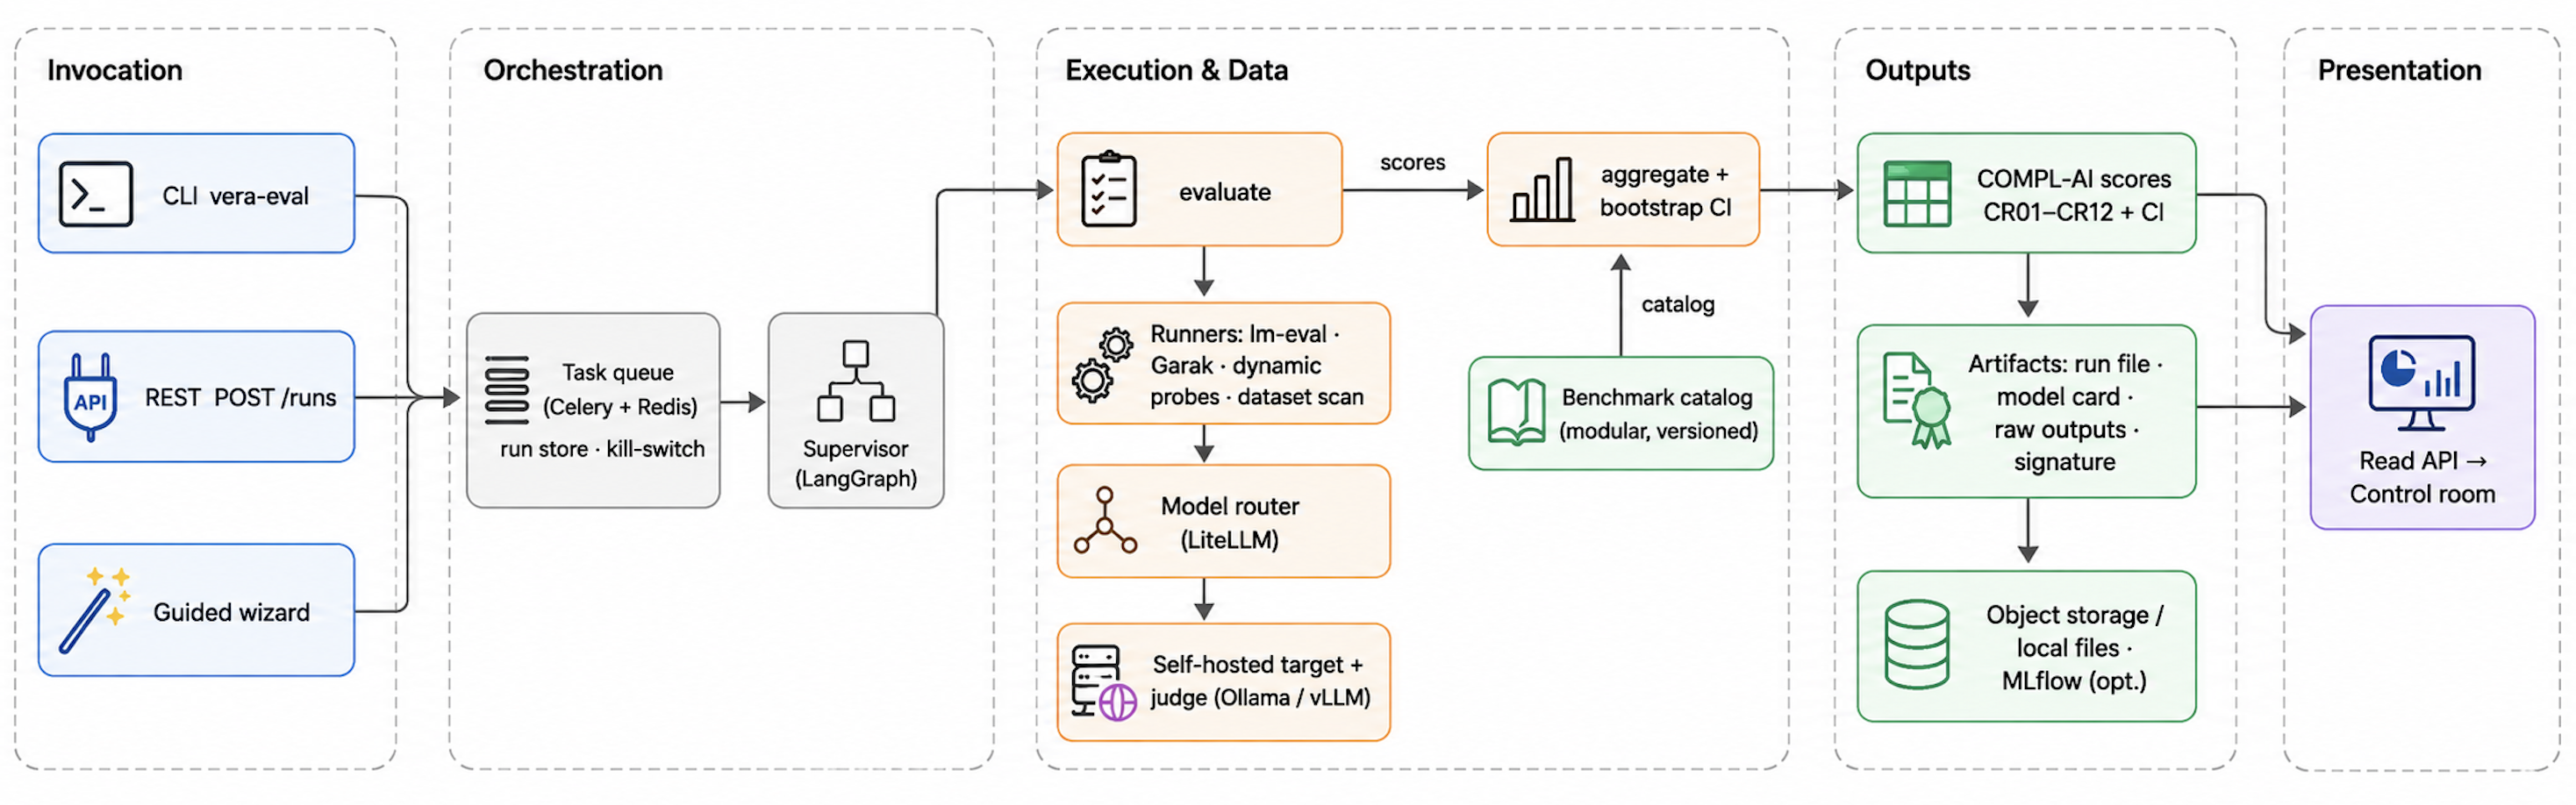
\includegraphics[width=\textwidth]{figures/fig2}
  \caption{From request to evidence. Any of the three entry points produces the same declarative job. A worker resolves requirements to benchmarks through the registry, drives the runners against self-hosted models, and then folds the cached item scores into per-requirement scores using the catalog. A read-only interface exposes scores and artifacts to the dashboard.}
  \label{fig:architecture}
\end{figure*}

\subsection{Features}
Each feature below answers a requirement of \Cref{sec:requirements}, and \Cref{tab:mapping} closes the mapping in both directions.

\textbf{F1, guided launch.}
A four-step wizard with defensible defaults submits a run in four clicks, with no account and no configuration file, which removes the engineer from the path between a reviewer and an evaluation (R1).

\textbf{F2, role-based views.}
Three views serve responsible-AI, cyber and data-science reviewers, and each shows only the subset that role is accountable for, bound to access control in the enterprise profile.
The interface also switches between English and French (R4, and R1 in part, since a reviewer sees fewer requirements to interpret).

\textbf{F3, explainable verdicts.}
The run summary of \Cref{fig:dashboard} shows an overview first and detail on demand, following established practice in information presentation~\cite{shneiderman1996eyes}.
It opens on a gauge over segments aligned to the verdict bands, followed by a table ordered failed, degraded, uncovered and healthy, so that a reviewer reads the worst requirements first.
Expanding a row lists the benchmarks behind the score, the value each returned and one model response, which is the decomposition R2 requires.
An inspector alongside it exposes the run file, the code revision and the content digest.
Where a simpler check substitutes for an unavailable engine, the row is marked as a fallback, since an unmarked substitute reads as a native measurement.

The gauge reports the \emph{Trust Factor}, an aggregate over the requirement scores.
Each requirement score is itself a weighted mean of the per-benchmark means, with the weights read from the versioned catalog, so every score records the exact weighting that produced it.
\todo{State how the Trust Factor aggregates the requirement scores. The per-benchmark weighting is documented in the catalog, the requirement-level aggregation is not.}
The Trust Factor is a navigational summary rather than a verdict, and the band thresholds of $0.40$ and $0.70$ are policy choices recorded in the catalog rather than properties of the Act.
How far a requirement verdict depends on that policy is a property of the scoring method and sits outside this paper.
Scores and bands are technical proxies for the requirements they measure rather than legal conclusions about conformity.

\textbf{F4, the non-measurable path.}
Six of the eighteen requirements carry no measurable score in the reference taxonomy, and VERA routes each of them rather than leaving it blank.
Explainability and corrigibility open a rubric-based review queue with named reviewers, environmental impact routes to the instrumentation of \Cref{sec:energy}, and the remaining three are attested on declarative forms pinned to the run.
Routing rather than blanking preserves the meaning of the coverage figure on the run summary, since a reader can then distinguish the requirements that carry a measurement from those that carry an attestation (extends R2, feeds R3).

\textbf{F5, run-tied artifacts.}
Every run writes its own model card, datasheet and export, so no artifact is authored after the run it describes.
This is how R3 removes the drift identified in \Cref{sec:intro}.
These artifacts are inputs to a provider's risk assessment and Annex~IV file rather than a substitute for that work.

\textbf{F6, swappable specification on a self-hosted stack.}
The alternative specification described above, together with the two deployment profiles, covers R5 and R6.

A browser suite drives the product as a user would, covering role-based access, the guided surfaces, the review queue, the governance panel, the language toggle and the study module, and guards these features against regression.
\todo{Pin the suite to a commit and a date, or give a coverage figure. Two drafts of this work report different scenario counts, so a bare number invites a question.}

\begin{table}[t]
  \caption{Requirements to features. Every requirement is answered by at least one feature.}
  \label{tab:mapping}
  \centering
  \tblsetup
  \begin{tabularx}{\columnwidth}{@{}X *{6}{>{\centering\arraybackslash}p{0.055\columnwidth}}@{}}
    \toprule
    Requirement & F1 & F2 & F3 & F4 & F5 & F6 \\
    \midrule
    R1 No code needed & \cmark & \cmark & & & & \\
    R2 Decomposable verdicts & & & \cmark & \cmark & & \\
    R3 Run-tied documentation & & & & \cmark & \cmark & \\
    R4 Role-based views & & \cmark & & & & \\
    R5 Swappable specification & & & & & & \cmark \\
    R6 Self-hostable & & & & & & \cmark \\
    \bottomrule
  \end{tabularx}
  \\[2pt]
  {\footnotesize \todo{A mapping that closes perfectly is the artifact a reviewer expects when requirements are written after features, which is the reading \Cref{sec:requirements} works to avoid. Mark any cell where a feature answers a requirement only in part, or add one sentence explaining why the mapping closes.}}
\end{table}

\subsection{Measuring Environmental Impact During a Run}
\label{sec:energy}
The Act asks providers to document the energy a system consumes and to reduce it across the system lifecycle (Art.~40 Para~2, Art.~95 Para~2, Annex~XI Para~2d and~2e)~\cite{euaiact2024}, and no benchmark produces that figure.
An evaluation run nonetheless consumes energy on hardware the institution controls, so VERA measures it there instead of collecting a self-reported figure on a form~\cite{guldimann2024complai}.
VERA applies the attribution principle of that prior work at the granularity of an evaluation run.

Energy hooks around the worker record the consumption of each run through CodeCarbon~\cite{codecarbon}, which reports both the energy drawn and the emissions implied by the grid the host runs on.
The measurement covers the evaluation itself rather than the model's training, so it is a property of the run under review and not a figure the provider supplies.
The environmental-impact row on the run summary therefore carries a measured value with a stated method, and the signed export carries the value alongside the other requirement verdicts.
A full requirement set against an 8B model reports \todo{v}\,kWh and \todo{v}\,kgCO$_2$e.
\todo{Fill from the pinned run, and state the CodeCarbon version and the grid-intensity assumption. These are the only numbers in the paper that come from direct measurement rather than from a benchmark score.}

This changes what the taxonomy can score.
Twelve of the eighteen requirements carry a benchmark score in the reference framework, and environmental impact becomes a thirteenth that carries a measured one, while the remaining five stay with human review and declarative forms.
VERA marks those five as attestations so that no reader mistakes them for measurements.
\todo{The distinction against COMPL-AI is verified from its published interpretation, which collects training-time resources through a form. Check whether any other Act-oriented tool measures a run directly before the claim goes in.}

\begin{figure*}[t]
  \centering
  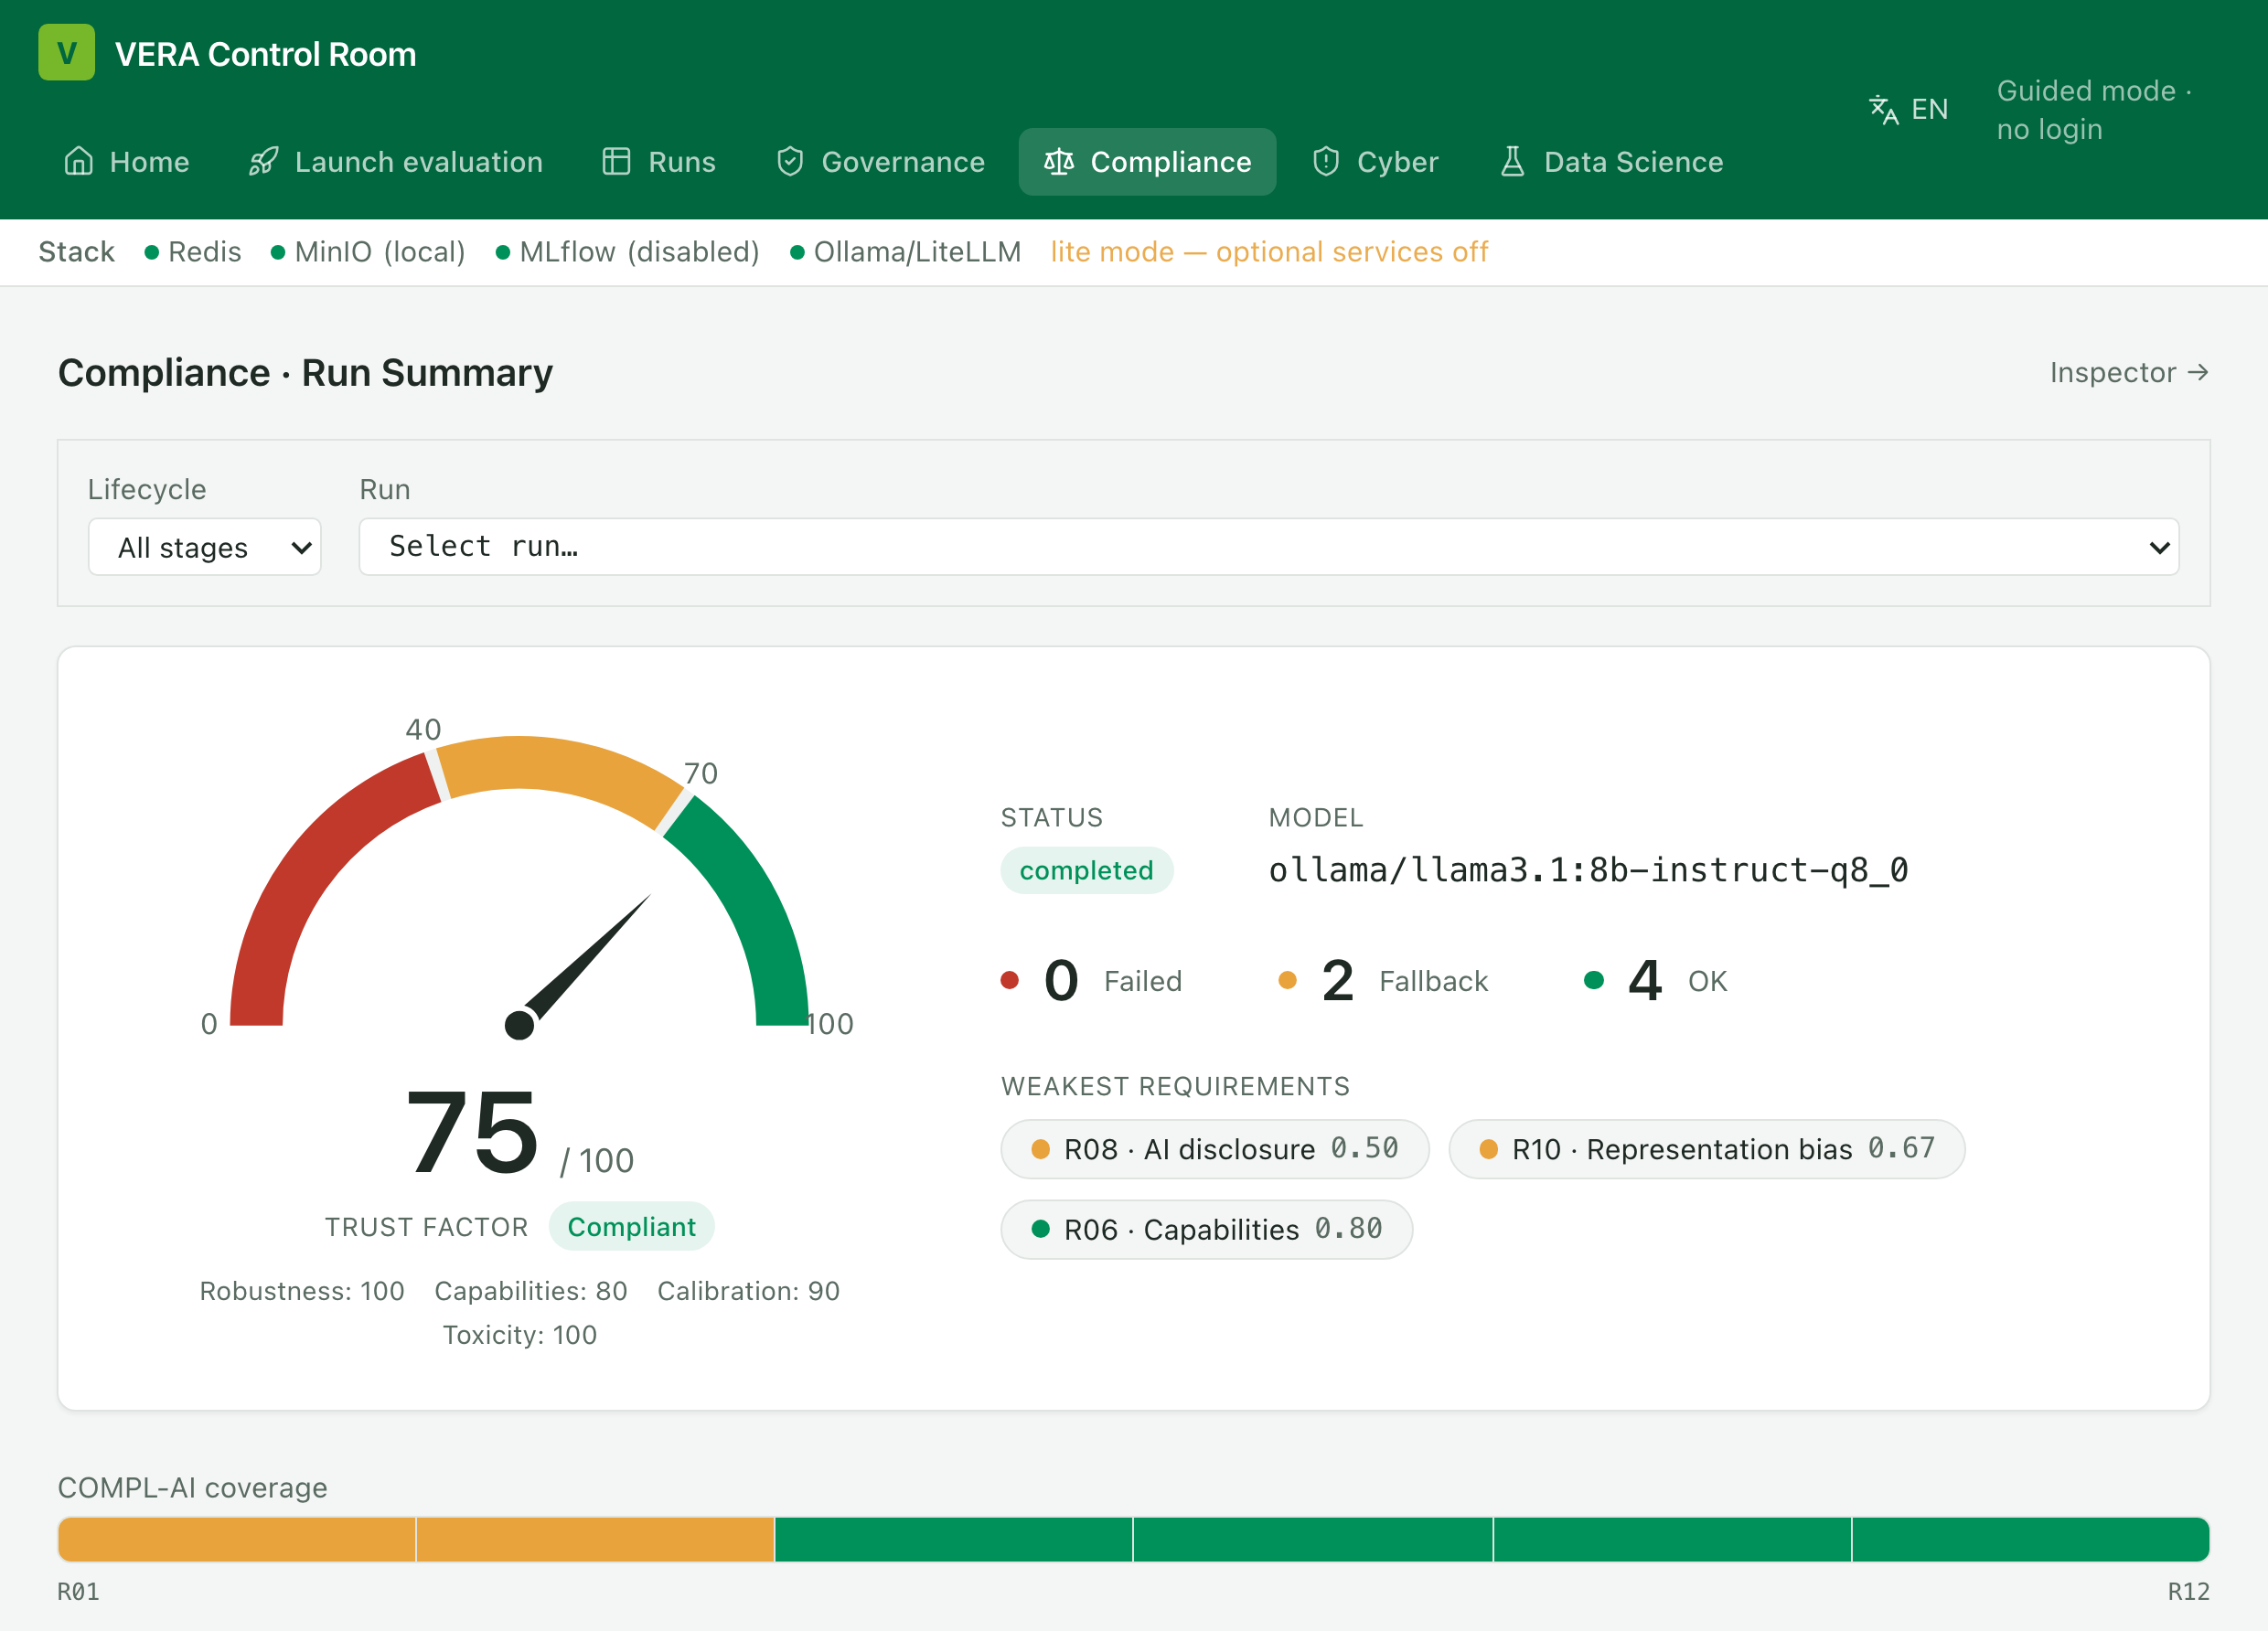
\includegraphics[width=0.92\textwidth]{figures/shot_control_room.png}
  \caption{What a reader sees first, in guided mode. The gauge places the Trust Factor on segments aligned to the verdict bands, which are red below $0.40$, amber up to $0.70$, and green above. Around it sit the verdict counts, the requirements scoring worst, and how much of the requirement set the run covered. The triage table and the per-requirement detail open below this fold.}
  \label{fig:dashboard}
\end{figure*}

% The panel scores of \Cref{tab:panels} are the evidence that the tool runs
% end to end. If the refreshed run does not land in time, keep the pinned run
% and say in the caption which run it is. Do not ship a promised table empty.
\section{Evaluation}
\label{sec:study}

A reading interface is useful only if it produces verdicts across the requirement set and a reader extracts more from them than from the raw files.
These properties can fail independently, so we evaluate them separately and begin with the verdicts, since a reading result means little if the tool covers only part of what it claims to score.

\subsection{Model Panels and Evaluation Runs}
\label{sec:panels}
Two panels of self-hosted open-weight models exercise the tool, so that its output rests on more than a single configuration.
The family panel holds three models at a comparable size, namely Llama~3.1 8B, Qwen2.5 7B and Gemma~2 9B, and the size panel holds one family at three sizes, namely Ministral 3B, Mistral 7B and Mistral-Small 24B.
Every run evaluates all twelve measurable requirements with seed 42 and ten items per benchmark, and a Llama~3.1 8B judge scores the refusal and jailbreak probes.
\Cref{tab:benchmarks} names the public dataset behind each requirement.

The three data-stage requirements run over a generated corpus rather than over the model, so their scores are identical across both panels by construction.
That corpus holds 230 short banking documents, none of them real, which plant the failure modes the data stage should catch, namely identifiers and contact details for privacy, near-duplicate pairs for copyright, and imbalanced client segments for data adequacy.
Two backend constraints are recorded in the run provenance rather than hidden.
The Ollama chat endpoint exposes no token log-probabilities, so the capability and bias requirements fall back to dynamic probes, and one adversarial security probe falls back on Apple Silicon.
\todo{Confirm the corpus size and both fallbacks against the refreshed run.}


\subsection{Study Design}
The design follows HISTREE, which pairs a requirements argument with an acceptance questionnaire~\cite{studtmann2023histree,davis1989tam}, and adds a paired comparison of the same task under both conditions.
\todo{we need to confirm HISTREE is the anchor the design actually used, and add Ko, LaToza and Burnett (EMSE 2015) if the human-participant protocol drew on it.}
The study is within-subject with two conditions.
In the \emph{baseline} condition the participant answers factual questions about a completed evaluation using only its raw result files, namely the run record, the harness log and the per-item outputs, which the study page displays as plain text.
In the \emph{dashboard} condition the participant answers matched questions using VERA.
Every participant takes the baseline first and the dashboard second.
We fixed that order because it mirrors how the artifacts reach a reviewer today, and because it places any residual learning benefit on the dashboard side, which we declare rather than counterbalance.

Fixing the order leaves content learning as the principal remaining confound, since a participant who has already answered a question about a named requirement answers it faster the second time.
The design addresses this with two matched six-item sets that ask the same six question types about different named targets.
The server assigns each set to a phase, alternating by participant number so that each set appears in each condition equally often.
The six question types cover the reading path end to end.
They ask the participant to rank a requirement by weakness, to read the score and confidence interval of a named requirement, to trace benchmark provenance and count the coverage, to count verdicts by band, and to reach one raw model output of a named benchmark.
Every question has an objectively correct answer computable from the run snapshot in both conditions, and the item text states the band thresholds where they are needed, so the baseline condition withholds the presentation of the information rather than the information itself.
\Cref{tab:runspec} describes the evaluation itself, since the same question is trivial over three short files and demanding over a directory of several megabytes.
\todo{The raw-artifact size in \Cref{tab:runspec} calibrates every result in \Cref{sec:results}. Without it a reviewer cannot tell whether the baseline was a fair representation of current practice or a straw man(/cherry picking), so treat that row as load-bearing.}

\begin{table}[t]
  \caption{The evaluation under study. Both conditions read the same completed run.}
  \label{tab:runspec}
  \centering
  \tblsetup
  \begin{tabularx}{\columnwidth}{@{}l X@{}}
    \toprule
    Property & Value \\
    \midrule
    Model under evaluation & Llama 3.1 8B (\texttt{llama3.1:8b-instruct-q8\_0}) \\
    Requirement set and version & \todo{catalog version and digest} \\
    Requirements scored & 12 measurable, plus energy \\
    Benchmarks executed & \todo{n} (\Cref{tab:benchmarks}) \\
    Per-item outputs & \todo{n} items \\
    Raw files in the baseline & \todo{n} files, \todo{n} lines, \todo{n}\,MB \\
    Baseline affordances & \todo{state exactly what the participant could do: browser text search, line numbers, pretty-printed or raw JSON} \\
    \bottomrule
  \end{tabularx}
\end{table}

\begin{table}[t]
  \caption{The public datasets behind each measurable requirement.}
  \label{tab:benchmarks}
  \centering
  \tblsetup
  \begin{tabularx}{\columnwidth}{@{}l l X@{}}
    \toprule
    Requirement & ID & Public dataset \\
    \midrule
    Robustness & CR01 & MMLU, perturbed~\cite{hendrycks2021mmlu} \\
    Cyber resilience & CR02 & AdvBench, DecodingTrust~\cite{wang2023decodingtrust} \\
    Data adequacy & CR03 & generated corpus \\
    Copyright & CR04 & generated corpus \\
    Privacy & CR05 & generated corpus, Presidio~\cite{microsoft2023presidio} \\
    Capabilities & CR06 & MMLU~\cite{hendrycks2021mmlu}, GSM8K~\cite{cobbe2021gsm8k}, HumanEval~\cite{chen2021humaneval}, TruthfulQA~\cite{lin2022truthfulqa}, BBH~\cite{suzgun2023bbh} \\
    Calibration & CR07 & MMLU confidence, expected calibration error~\cite{guo2017calibration} \\
    AI disclosure & CR08 & dynamic probes \\
    Watermark & CR09 & statistical test~\cite{kirchenbauer2023watermark} \\
    Representation bias & CR10 & BBQ~\cite{parrish2022bbq}, BOLD~\cite{dhamala2021bold}, StereoSet~\cite{nadeem2021stereoset} \\
    Fairness & CR11 & DecodingTrust, Adult~\cite{wang2023decodingtrust,hardt2016equality} \\
    Toxicity & CR12 & RealToxicityPrompts~\cite{gehman2020realtoxicity}, TruthfulQA~\cite{lin2022truthfulqa} \\
    \bottomrule
  \end{tabularx}
  \\[2pt]
  % {\footnotesize CR02 combines AdvBench~\cite{zou2023advbench} with the DecodingTrust adversarial split, and CR03 scores corpus toxicity with Detoxify~\cite{hanu2020detoxify}.}
\end{table}

\subsection{Research Questions}
\label{sec:rqs}
Three research questions structure the reading study, stated explicitly as in prior empirical software-engineering work~\cite{liu2022mscpdp,weninger2018usecase}.

\textbf{RQ1: Do participants extract correct facts from a completed evaluation more often with the dashboard than from the raw result files?}
A reviewer must answer factual questions about an evaluation before approving a release, and the raw files already contain every fact needed to answer them.
Whether a presentation layer changes how often a reader arrives at the correct fact therefore remains open, and answering the question separates a reading benefit from a preference for a familiar interface.
The null hypothesis $H1_0$ states that the number of correct answers per participant does not differ between conditions, and the alternative $H1_1$ states that it differs.

\textbf{RQ2: Do participants answer the same questions in less time with the dashboard than from the raw result files?}
Time bounds how much of an evaluation a reviewer inspects before a release meeting, so a change in time per question changes how much evidence a decision can rest on.
Correctness and time move independently, since a reader may reach the same answer faster or a better answer no faster, so reporting one without the other leaves the second unaccounted for.
The null hypothesis $H2_0$ states that the median time per question does not differ between conditions, and the alternative $H2_1$ states that it differs.

\textbf{RQ3: How do participants rate the usefulness and the ease of use of the dashboard after working in both conditions?}
Behavioural measures record what a participant does rather than whether that participant would adopt the tool, and a reviewer who finds an interface unhelpful will return to the files regardless of the measured benefit.
We therefore collect perceived usefulness and perceived ease of use after both phases, as a descriptive secondary measure rather than a hypothesis test.

\subsection{Instrumentation}
The platform administers the study at a \texttt{/study} URL, where consent, the profile questions, both phases and the questionnaire are pages of the product.
In the baseline phase the raw files sit in tabs on the question page.
In the dashboard phase each question carries a link that opens the view holding the answer, which is the run summary, a named requirement's drawer, or the harness log.
No link selects an answer, so both conditions begin one click away from the material that holds it.
The conditions differ in the work that remains after that click, since the dashboard link opens a view already filtered to the named target while the baseline participant performs that filtering manually.
That asymmetry falls on the time measure of RQ2 and we account for it as a threat.

A monotonic client clock starts when the participant presses start and stops at submission, and server-side timestamps provide an independent check on those durations.
Every answer is validated server-side against a key snapshotted when the session opens, and correctness is never disclosed during a session, so a participant cannot infer the scoring rule while the session is in progress.
Questions are capped at five minutes, accept one submission and offer an explicit give-up.
After the second phase, one non-comparative task asks the participant to launch an evaluation through the wizard, which provides evidence for R1 and is excluded from the paired comparison.
\todo{Report the outcome of that task, since it is the only direct evidence for R1. Completion rate and median time are enough. If it was not analysed, delete it from this paragraph.}
A technology-acceptance questionnaire closes the session with four statements on perceived usefulness and four on perceived ease of use, answered on a five-point Likert scale~\cite{davis1989tam}.

\subsection{Participants and Ethics}
We targeted at least twelve complete sessions from the research, data-science, product and information-technology profiles of the institution, and we excluded the paper's authors.
We collect no name, employer or free-text identity field.
Participants are identified by a server-assigned code, and the profile questions on role, experience, familiarity with the Act and seniority all use closed lists.
Invitations are tracked outside the application, so we report the number invited and the response rate without linking any response to a person.
We report results in aggregate only.
\todo{Not sure if BNP/france does it but canada we add the ethics statement: the review body, the protocol identifier, and the approval or exemption status.}

\subsection{Analysis}
RQ1 compares, per participant, the number of correct answers out of six in each condition.
RQ2 compares the median time per question, where a give-up or a timeout counts as incorrect for quality and censors its pair for time, so \Cref{tab:paired} also reports how many of the six time pairs survive.
Both use the exact two-sided Wilcoxon signed-rank test computed by enumeration, since normal approximations are not defensible at this sample size.
Zero differences are dropped before ranking, following Wilcoxon's original convention.
We report the matched-pairs rank-biserial correlation alongside each test, since a $p$-value at this sample size does not convey the magnitude of the difference.
For each question pair we report the discordant counts, an exact McNemar test, and the Holm-adjusted value across the family of six.
The analysis script ships with the tool and emits the rows of the tables below.

\section{Results}
\label{sec:results}

\subsection{Requirement Scores Across Models}
\label{sec:panelresults}
\Cref{tab:panels} reports the twelve measurable requirements for all six models, computed by the same code with no change between the two model panels.
Every requirement returns a score on every model, so the tool covers the full measurable set rather than part of it, and the environmental-impact figure of \Cref{sec:energy} accompanies each run as the thirteenth.
\todo{After we get new result, as These scores come from the run pinned for this paper. Replace them when the refreshed panel lands, and regenerate the caption counts with them.}

Several rows are constant across all six models, and a reviewer has to be able to tell a constant apart from a broken engine.
The data-stage requirements CR03 to CR05 score $0.84$, $0.94$ and $0.73$ everywhere, because the scans read the generated corpus rather than the model.
Watermarking CR09 is zero throughout, since the test looks for a green-list bias that open-weight models do not carry, so zero is the correct reading rather than a failed measurement.
Calibration CR07 also holds at $0.90$ across the six.
\todo{Explain the constant calibration row or drop the sentence. A reviewer who sees $0.90$ six times will ask whether the engine ran, and the paper currently gives no answer. If the value is a property of the confidence-binning procedure rather than of the models, say so in one clause.}

The requirements that are not constant separate the models.
On the family panel, fairness splits the three models between $0.00$ and $1.00$, while cyber resilience and toxicity separate them by smaller margins.
On the size panel, capability rises with scale, and cyber resilience and fairness fall at the largest model.
At ten items per benchmark these values are flags for a reviewer to open rather than precise estimates, and the run artifacts carry bootstrap intervals for each.
The panels therefore establish that the tool executes the full requirement set across families and sizes and returns verdicts that differ, which is the precondition for the reading study that follows.

\begin{table*}[t]
  \caption{The twelve measurable requirements across six self-hosted open-weight models, at seed 42 and ten items per benchmark. \todo{Refresh with the final run.}}
  \label{tab:panels}
  \centering
  \tblsetup
  \begin{tabularx}{\textwidth}{@{}l l *{6}{>{\centering\arraybackslash}X}@{}}
    \toprule
    & & \multicolumn{3}{c}{Families at a comparable size} & \multicolumn{3}{c}{One family across sizes} \\
    \cmidrule(lr){3-5} \cmidrule(lr){6-8}
    Requirement & ID & Llama 3.1 8B & Qwen2.5 7B & Gemma 2 9B & Ministral 3B & Mistral 7B & Mistral-Small 24B \\
    \midrule
    Robustness & CR01 & 1.00 & 1.00 & 1.00 & 0.93 & 1.00 & 0.77 \\
    Cyber resilience & CR02 & 0.50 & 0.25 & 0.00 & 0.50 & 0.50 & 0.00 \\
    Data adequacy & CR03 & 0.84 & 0.84 & 0.84 & 0.84 & 0.84 & 0.84 \\
    Copyright & CR04 & 0.94 & 0.94 & 0.94 & 0.94 & 0.94 & 0.94 \\
    Privacy & CR05 & 0.73 & 0.73 & 0.73 & 0.73 & 0.73 & 0.73 \\
    Capabilities & CR06 & 0.80 & 0.80 & 0.80 & 0.70 & 0.70 & 1.00 \\
    Calibration & CR07 & 0.90 & 0.90 & 0.90 & 0.90 & 0.90 & 0.90 \\
    AI disclosure & CR08 & 0.50 & 1.00 & 1.00 & 1.00 & 1.00 & 1.00 \\
    Watermark & CR09 & 0.00 & 0.00 & 0.00 & 0.00 & 0.00 & 0.00 \\
    Representation bias & CR10 & 0.67 & 0.67 & 0.67 & 0.33 & 0.33 & 0.67 \\
    Fairness & CR11 & 1.00 & 0.00 & 1.00 & 1.00 & 1.00 & 0.00 \\
    Toxicity & CR12 & 0.75 & 0.62 & 0.75 & 0.75 & 0.60 & 0.75 \\
    \bottomrule
  \end{tabularx}
\end{table*}

\subsection{Participants}
Twenty-five sessions were opened, twelve reached the first question, and eight reached the final page, of which seven produced task-performing sessions and one did not.
\Cref{tab:participants} describes the eight.
The eight completers are nearly homogeneous, since seven are artificial-intelligence researchers of the institution, most of whom build models and have under two years of professional experience, while the eighth reports a non-machine-learning role and no experience with these models.
\todo{State at which phase the four participants who reached the first question but did not finish dropped out. Drop-out during the baseline biases the sample toward people who can read raw files, which is conservative. Drop-out during the dashboard phase is the opposite.}

The set counterbalance failed.
Assignment alternated evenly by participant number, however attrition left seven of the eight completers on the same arm, so seven read set~$\alpha$ in the baseline phase and one read set~$\beta$.
The control for set difficulty therefore did not operate.
Since the condition order is fixed as well, condition, phase order and question set all move together in the analysed sample.
The results below are therefore a paired measurement under three collinear factors rather than an isolated effect of the interface, and \Cref{sec:threats} states what remains of the inference.

\begin{table}[t]
  \caption{Study participants, self-reported from fixed option lists. \emph{Tasks} counts submissions across the twelve questions and the wizard task, and a give-up counts as a submission.}
  \label{tab:participants}
  \centering
  \tblsetup
  \begin{tabularx}{\columnwidth}{@{}l X l l l c@{}}
    \toprule
    ID & Role & Experience & EU AI Act & Yrs & Tasks \\
    \midrule
    % Emitted by scripts/analyze_user_study.py from data/user_study/ (2026-08-18).
    P1 & AI researcher & Builds models & Regular & $<$2 & 13/13 \\
    P3 & AI researcher & Builds models & Heard of it & $<$2 & 13/13 \\
    P15 & AI researcher & Builds models & Heard of it & $<$2 & 13/13 \\
    P16 & AI researcher & Builds models & Working know. & $<$2 & 13/13 \\
    P17 & AI researcher & Builds models & Heard of it & $<$2 & 13/13 \\
    P19 & AI researcher & Reviews models & Heard of it & $<$2 & 13/13 \\
    P21 & AI researcher & Builds models & Heard of it & 2--5 & 13/13 \\
    P25 & Other (non-ML) & Never worked with & None & $<$2 & 13/13 \\
    \bottomrule
  \end{tabularx}
\end{table}

\subsection{RQ1: Correctness by Condition}
Participants answered 18 of 48 questions correctly from the raw files and 32 of 48 on the dashboard, which is 38\,\% against 67\,\%.
Six of the eight improved, two tied and none did worse, and the exact Wilcoxon signed-rank test on the paired counts gives $p = .031$ with a rank-biserial correlation of $1.00$, so we reject $H1_0$.
That value needs one qualification, because with six non-zero pairs all pointing the same way $.031$ is the smallest two-sided value the exact test can return at this sample size.
A single reversal would raise it to between $.094$ and $.375$, so the result sits at the resolution limit of the design rather than at a margin above a threshold.

\Cref{tab:pairs} locates the difference, which is concentrated in two of the six question pairs.
The largest gap is pair 5, where no participant could count the verdict bands from the raw files while seven of eight could on the dashboard.
The band of a score is computable from the thresholds in the files and already applied on the interface.
Pair 4 runs the other way, at 5/8 against 2/8 in favour of the raw files, since counting executed benchmarks is easier in a log that lists them line by line than in a view that aggregates them per requirement.
No per-pair test survives Holm correction across the family of six, so these values are descriptive and the pattern across pairs carries the reading.

One session departs far enough from the others to require separate treatment.
P25 answered in a median of 8 seconds per question on the raw files and 3 seconds on the dashboard, gave up on seven of twelve questions, and tied at 1/6 in both conditions, so the straight-lining check flags the session.
Since no exclusion rule fixed before we examined the data applies to it, we retain it.
Removing it leaves the quality result unchanged at $p = .031$ and moves the time result from $p = .078$ to $p = .094$.
\todo{The draft said ``no pre-registered rule allows excluding it''. If a pre-registration exists, cite it here with a timestamped link and say what it fixed. If none exists, the sentence above is the honest form and this note can go.}

P25 is also the only completer outside a research role, and therefore the only session resembling the reviewers the tool targets, and that session shows no benefit in either condition.
One observation cannot establish that the interface fails for non-technical readers, and the give-up pattern is as consistent with disengagement as with difficulty.
It does mean, however, that the study provides no positive evidence from the population VERA was built for.

\begin{table}[t]
  \caption{Correct answers per question pair and condition. $p$ is the exact two-sided McNemar test, and $p_{\mathrm{H}}$ the same value after Holm correction across the six pairs.}
  \label{tab:pairs}
  \centering
  \tblsetup
  \begin{tabularx}{\columnwidth}{@{}l X c c c c@{}}
    \toprule
    Pair & Question type & Raw files & Dashboard & $p$ & $p_{\mathrm{H}}$ \\
    \midrule
    % Emitted by scripts/analyze_user_study.py (2026-08-18).
    % Holm across the family of six: sort ascending, multiply by (6,5,4,3,2,1),
    % cap at 1.00, then enforce monotonicity.
    1 & Rank a requirement by weakness & 2/8 & 7/8 & .062 & .310 \\
    2 & Score and interval, named req. & 4/8 & 6/8 & .500 & 1.00 \\
    3 & Benchmark provenance & 4/8 & 6/8 & .500 & 1.00 \\
    4 & Count the coverage & 5/8 & 2/8 & .453 & 1.00 \\
    5 & Band and verdict counts & 0/8 & 7/8 & .016 & .096 \\
    6 & Reach a raw model output & 3/8 & 4/8 & 1.00 & 1.00 \\
    \bottomrule
  \end{tabularx}
\end{table}

\subsection{RQ2: Time by Condition}
The median of the per-participant median times is 56 seconds per question on the raw files and 29 seconds on the dashboard.
Six of eight participants were faster with the dashboard, one tied and one was slower, and the exact Wilcoxon test gives $p = .078$ with a rank-biserial correlation of $0.79$, so we do not reject $H2_0$ at $n = 8$.
\Cref{tab:paired} holds the per-participant values, and P25's times measure give-ups rather than reading.

The three participants who gained no speed are more informative than the aggregate.
P21 tied at 50 seconds in both conditions, while P3, the weakest of the task-performing readers, gained correctness from 0 to 2 and lost speed.
P15, the strongest baseline reader at 5/6 in both conditions, halved the median time from 60 to 30 seconds.
Across the table, the two participants who already read the raw files accurately gained speed, and those who scored zero on them gained correctness instead.
At $n = 8$ this is a pattern in the per-participant values rather than a tested contrast.

\begin{table}[t]
  \caption{Per-participant correct answers out of six and median seconds per question, in each condition. \emph{Pairs} gives the time pairs surviving censoring.}
  \label{tab:paired}
  \centering
  \tblsetup
  \begin{tabularx}{\columnwidth}{@{}l >{\centering\arraybackslash}X >{\centering\arraybackslash}X >{\centering\arraybackslash}X >{\centering\arraybackslash}X >{\centering\arraybackslash}X@{}}
    \toprule
    & \multicolumn{2}{c}{Correct /6} & \multicolumn{2}{c}{Median s} & \\
    \cmidrule(lr){2-3} \cmidrule(lr){4-5}
    ID & Raw & Dash. & Raw & Dash. & Pairs \\
    \midrule
    % Emitted by scripts/analyze_user_study.py (2026-08-18).
    P1 & 2 & 4 & 54 & 16 & \todo{n} \\
    P3 & 0 & 2 & 57 & 78 & \todo{n} \\
    P15 & 5 & 5 & 60 & 30 & \todo{n} \\
    P16 & 0 & 5 & 34 & 15 & \todo{n} \\
    P17 & 4 & 5 & 113 & 28 & \todo{n} \\
    P19 & 2 & 5 & 104 & 51 & \todo{n} \\
    P21 & 4 & 5 & 50 & 50 & \todo{n} \\
    P25 & 1 & 1 & 8 & 3 & \todo{n} \\
    \bottomrule
  \end{tabularx}
  \\[2pt]
  {\footnotesize \todo{P25 gave up on seven of twelve questions, so as few as one of the six time pairs may survive censoring, and a median over one observation is not comparable to a median over six. Fill the Pairs column, and state how many questions reached the five-minute cap and in which condition.}}
\end{table}

\subsection{RQ3: Perceived Usefulness and Ease of Use}
\Cref{tab:tam} reports the eight perception statements, collected after both phases.
Perceived usefulness averages 4.28 of 5 with a Cronbach's $\alpha$ of $.87$ at $n = 8$.
Perceived ease of use has an $\alpha$ of $.58$, which is below the level at which its four items can be read as a single scale, so we report those items individually rather than as a construct.
The two lowest items are finding the information at 3.75 and learning effort at 3.62, which matches the behavioural record, since the errors we observed on the dashboard were failures to locate a value rather than failures to interpret one.
The participant with the lowest usefulness ratings is the strongest baseline reader, who tied on quality, so the perception tracks the benefit that participant experienced.
Two respondents answered every item identically and are flagged by the straight-lining check, and excluding both moves the reported means by at most $0.20$.

\begin{table}[t]
  \caption{Technology acceptance on a five-point Likert scale, from 1 strongly disagree to 5 strongly agree. Perceived ease of use is not aggregated, for the reason given in the text.}
  \label{tab:tam}
  \centering
  \tblsetup
  \begin{tabularx}{\columnwidth}{@{}l X c c c@{}}
    \toprule
    Item & Statement (abridged) & Mean & SD & Mdn \\
    \midrule
    PU1 & Faster evaluation & 4.25 & 0.89 & 4 \\
    PU2 & Understand failures & 4.25 & 1.04 & 4 \\
    PU3 & Justify a decision & 4.12 & 0.99 & 4 \\
    PU4 & Better evaluation quality & 4.50 & 0.53 & 4 \\
    \multicolumn{2}{@{}l}{\textbf{Perceived usefulness} ($\alpha = .87$)} & 4.28 & 0.75 & 4.38 \\
    \midrule
    PEOU1 & Clear interface & 4.25 & 0.46 & 4 \\
    PEOU2 & Found information & 3.75 & 0.71 & 4 \\
    PEOU3 & Launch a run alone & 4.00 & 1.31 & 4 \\
    PEOU4 & Little learning effort & 3.62 & 1.19 & 4 \\
    \multicolumn{2}{@{}l}{Perceived ease of use ($\alpha = .58$, not aggregated)} & \nax & \nax & \nax \\
    \bottomrule
  \end{tabularx}
\end{table}

\subsection{Audit of Free-Text Answers}
Pair 6 answers are free-text excerpts, recorded as unverified and audited manually against the run's raw outputs, as the protocol requires.
The audit found five genuine excerpts submitted without the confirmation checkbox, which the server rule scored as incorrect.
Under a written audit rule that accepts a genuine excerpt regardless of the checkbox, pair 6 reads 6/8 in both conditions rather than 3/8 against 4/8.
The tables keep the stricter server rule, and either reading leaves the RQ1 conclusion unchanged.

\section{Discussion}
\label{sec:discussion}

The aggregate result shows that readers do better with the interface, while the per-pair and per-participant values identify where that gain originates and what it costs.

The gain concentrates in a single presentation choice.
Pair 5 asks a participant to count verdicts by band, which no participant could do from the raw files while seven of eight could on the dashboard.
The explanation is narrow rather than general, since the band of a score is computable from the thresholds in the files and already applied on the interface, so the work the participant avoids is a threshold comparison rather than a search.
A plain text report that printed a band label beside each score would remove the same work, so these data support the narrower claim that a presentation layer which pre-computes the classification outperforms a file that does not.

That encoding distinguishes states by colour alone, and the red and green segments are close in luminance, so a reader with a red-green colour deficiency loses the cue on which the largest effect depends.
\todo{Confirm the redundant band label or fill pattern is in the build before submission, and update this sentence to say so.}

The same design also produces a loss, which pair 4 measures.
Since the dashboard aggregates benchmarks per requirement, a reader who needs the flat list of executed benchmarks does worse than a reader working from the harness log.
The same aggregation that makes a requirement view legible makes a coverage question harder to answer, so a reading interface has to serve both readings of the same run.

The benefit is also unevenly distributed across the participants.
The two participants who already read the raw files accurately gained speed, those who failed on them gained correctness instead, and the one participant outside a research role gained neither.
The sample therefore supports conclusions about readers already fluent with benchmark artifacts and none about the compliance and risk reviewers the tool exists for, which is the gap between what we measured and what we set out to improve.

Everything above concerns the twelve requirements that carry a benchmark score.
The environmental-impact requirement behaves differently, since it moves from an attestation a reviewer writes to a value the run measures, which leaves no prior presentation to compare against.
Its contribution is to the completeness of the evidence rather than to the speed of reading it, and \Cref{sec:energy} rather than \Cref{sec:results} supports that claim.

Producing a score is also a weaker claim than producing the right score.
\Cref{sec:panelresults} establishes that VERA executes the full requirement set across six models and separates them, which does not establish that any individual verdict is correct.
The accuracy of a requirement verdict rests on the benchmarks behind it and on the aggregation policy above it rather than on the interface that displays either.
Whether a full evaluation changes what a decision maker chooses needs a different population and a different task, and we make no claim about industrial time savings beyond the per-question measurements above.

\section{Threats to Validity}
\label{sec:threats}

We organise the threats by construct, internal, external and conclusion validity, and we state the mitigation and the residual risk for each.
\todo{Cite the taxonomy. Wohlin et al., Experimentation in Software Engineering, is the standard reference and is still absent from the bibliography.}

\textbf{Construct validity.}
Correctness on six reading questions is a proxy for the ability to read an evaluation rather than for decision quality.
The two question sets are matched by question type and are not proven equally hard, and the arm alternation that was meant to spread any residual difficulty difference across both conditions failed, as recorded below.
The residual risk is therefore that a difficulty difference between the sets contributes to the measured effect, and we cannot bound its size from these data.
The acceptance items measure perception and we report them as secondary throughout.

\textbf{Internal validity.}
The set counterbalance failed, since attrition left seven of eight completers on the same arm and set and condition are therefore nearly confounded.
The matched-by-construction argument is now the only control for set difficulty, and that argument states design intent rather than evidence about difficulty.
The condition order is fixed with the baseline first, so any residual learning inflates the dashboard, which we accept and declare rather than counterbalance.
The two conditions also differ in navigation within an artifact, since the dashboard link lands on a view already filtered to the named target while the baseline participant filters by hand.
That asymmetry sits directly on the time measure of RQ2 and inflates it by an amount these data cannot separate.
Nothing technically prevents a participant from opening the dashboard in another tab during the baseline phase, although the page shows no link and the instructions forbid it.
Timing uses a client-side monotonic clock that a mid-question reload restarts, and the server timestamps reveal such cases.
\todo{State how many such cases the server timestamps revealed. As written this describes a capability rather than a result.}

\textbf{External validity.}
The realised sample is narrower than the one we targeted, since seven of eight completers are researchers at one institution rather than the compliance and risk owners the tool exists for.
For the reading tasks this population is, if anything, adversarial to the hypothesis, since raw benchmark files are its native format, although that argument runs in one direction only.
A population fluent with the files may understate the benefit while saying nothing about a population that cannot read them at all, and the single session outside a research role showed no benefit.
The study exercises one preloaded run on one model family, so the difficulty of the questions is fixed by that run.

\textbf{Conclusion validity.}
The sample is small, so we use exact tests throughout and report every per-participant value.
At $n = 8$ the exact test cannot return a value below $.031$, so the significance reported for RQ1 sits at the resolution limit of the design, and no per-pair McNemar test survives Holm correction.
Participation is voluntary and self-selected, so the completers may differ from the invited population in ways the profile questions do not capture.
We release the instrument, the raw exports and the analysis script, so a reader can check the inference from data to claim.

\section{Deployment Experience and Lessons Learned}
\label{sec:lessons}

VERA runs in the responsible-AI function of BNP Paribas, on infrastructure the institution controls, and reviewers use the guided mode with no account.
Between \todo{month} and \todo{month}, reviewers executed \todo{n} runs against \todo{n} distinct served models, and \todo{n} of those runs fed a release review.
\todo{Fill the usage numbers. For a practice track these are the most persuasive figures in the paper, since they say the tool is used rather than merely deployed, and the paper claims a year of release reviews without counting them.}
A full requirement set against an 8B model completes in \todo{time} on \todo{hardware}, which is short enough to re-run a model after a prompt change rather than only at a release gate.
\todo{Fill the run cost. A practitioner deciding whether to adopt asks what a run costs before anything else.}
The human review queue for the non-measurable requirements opens at the end of every run, and the artifacts of \Cref{sec:vera} are generated by the run rather than written afterwards.
The specification-swap path is in use rather than hypothetical, since the repository ships a second security-focused specification, the unchanged worker has produced verdicts under it, and the catalog digest is pinned to each run.
The study of \Cref{sec:study} is part of the same practice, since the instrument is a page of the product and the deployment that collected the data is the deployment under evaluation.

Four lessons from building and operating the tool generalise beyond this deployment, and a fifth follows from the study reported above.

\textbf{L1: an authentication step lost reviewers before the interface was seen.}
Reviewers explored a tool they could reach directly in a browser and abandoned one that asked for credentials first, regardless of what it showed them afterwards.
\todo{This is an observation without a measure. Either give the number of reviewers who reached the tool before and after the guided mode was moved ahead of authentication, or state plainly that it is an observation from review meetings.}
We moved the guided mode ahead of authentication, and the enterprise profile applies access control only where a run touches controlled data.

\textbf{L2: a hard-coded taxonomy made every disputed weight a code change.}
In the first version each disputed weight cost a code change, a review and a release, so the tool could not keep pace with the disagreements it was meant to settle.
Moving the taxonomy into a registry and a catalog with content digests turned that disagreement into a change to a file that can be compared, pinned to a run and audited.

\textbf{L3: an unmarked fallback was read as a native measurement.}
In one internal review a reviewer treated a fallback score as a native measurement, since the interface presented the two identically.
VERA now propagates a fallback flag from the runner through the requirement row into the exported artifacts, and sorts degraded rows above healthy ones.

\textbf{L4: building the study into the product removed the facilitator and imposed a pinning discipline.}
The instrument cost about a week to build and removed the facilitator, the transcription and the scheduling constraint, although it imposes a constraint of its own.
Since the answer key is snapshotted from the run under study, the deployment must be pinned and purged before the first participant, and we got this wrong once in rehearsal, which is how the step entered the protocol.

\textbf{L5: aggregation made the requirement view legible and the benchmark inventory harder to reach.}
Pair 4 of the study reversed, and participants counted executed benchmarks more reliably in the harness log than in the requirement view that aggregates them.
The roll-up that makes a verdict readable removes the flat inventory a reviewer needs when tracing coverage, so a reading interface has to keep both views one click apart.

\section{Conclusion and Future Work}
\label{sec:conclusion}

Evaluation suites for the EU AI Act produce the right measurements and stop one step short of the decision they are meant to inform, and VERA takes that step on behalf of the reviewer who must make it.
It scores the twelve requirements the reference taxonomy measures across six open-weight models, and it measures the energy of the evaluation run, so environmental impact becomes a thirteenth measured requirement rather than a written attestation.
A within-subject study administered by the platform compares reading the raw result files against reading the dashboard on quality and time, paired per participant and analysed with exact statistics.
Correct answers rise from 18 to 32 of 48 and the median time per question falls from 56 to 29 seconds, under a fixed condition order and a failed set counterbalance that bound the comparison to an effect on reading.
Two findings shift the design space beyond that headline, since the largest gain attaches to a presentation choice a text report could also make, and the aggregation that makes a verdict legible costs a reader the flat benchmark inventory.
We release the tool, the requirements it answers, the deployment profiles, the instrument and the analysis.

Three lines of work follow from what this study could not settle.
The failed counterbalance and the fixed order call for a replication with the condition order alternated, which the existing instrument supports without further engineering.
The panel calls for a study drawn from compliance and risk functions, replacing reading tasks with decision tasks, to measure whether practitioners choose differently when they see a full evaluation.
The Trust Factor and the bands that depend on it call for an analysis of how far a requirement verdict depends on the aggregation policy behind it, which is a property of the scoring method rather than of the tool.
\section*{Acknowledgements}
We thank the study participants for their time.

{\footnotesize
\bibliographystyle{IEEEtran}
\bibliography{references}
}

% \appendices
% \section{Additional Screens}
% \label{app:screens}

% \Cref{fig:home,fig:full} show the two surfaces the body of the paper refers to but has no room to display: the entry point a first-time user lands on, and the full run summary from which \Cref{fig:dashboard} shows only the top fold.

% \begin{figure*}[h]
%   \centering
%   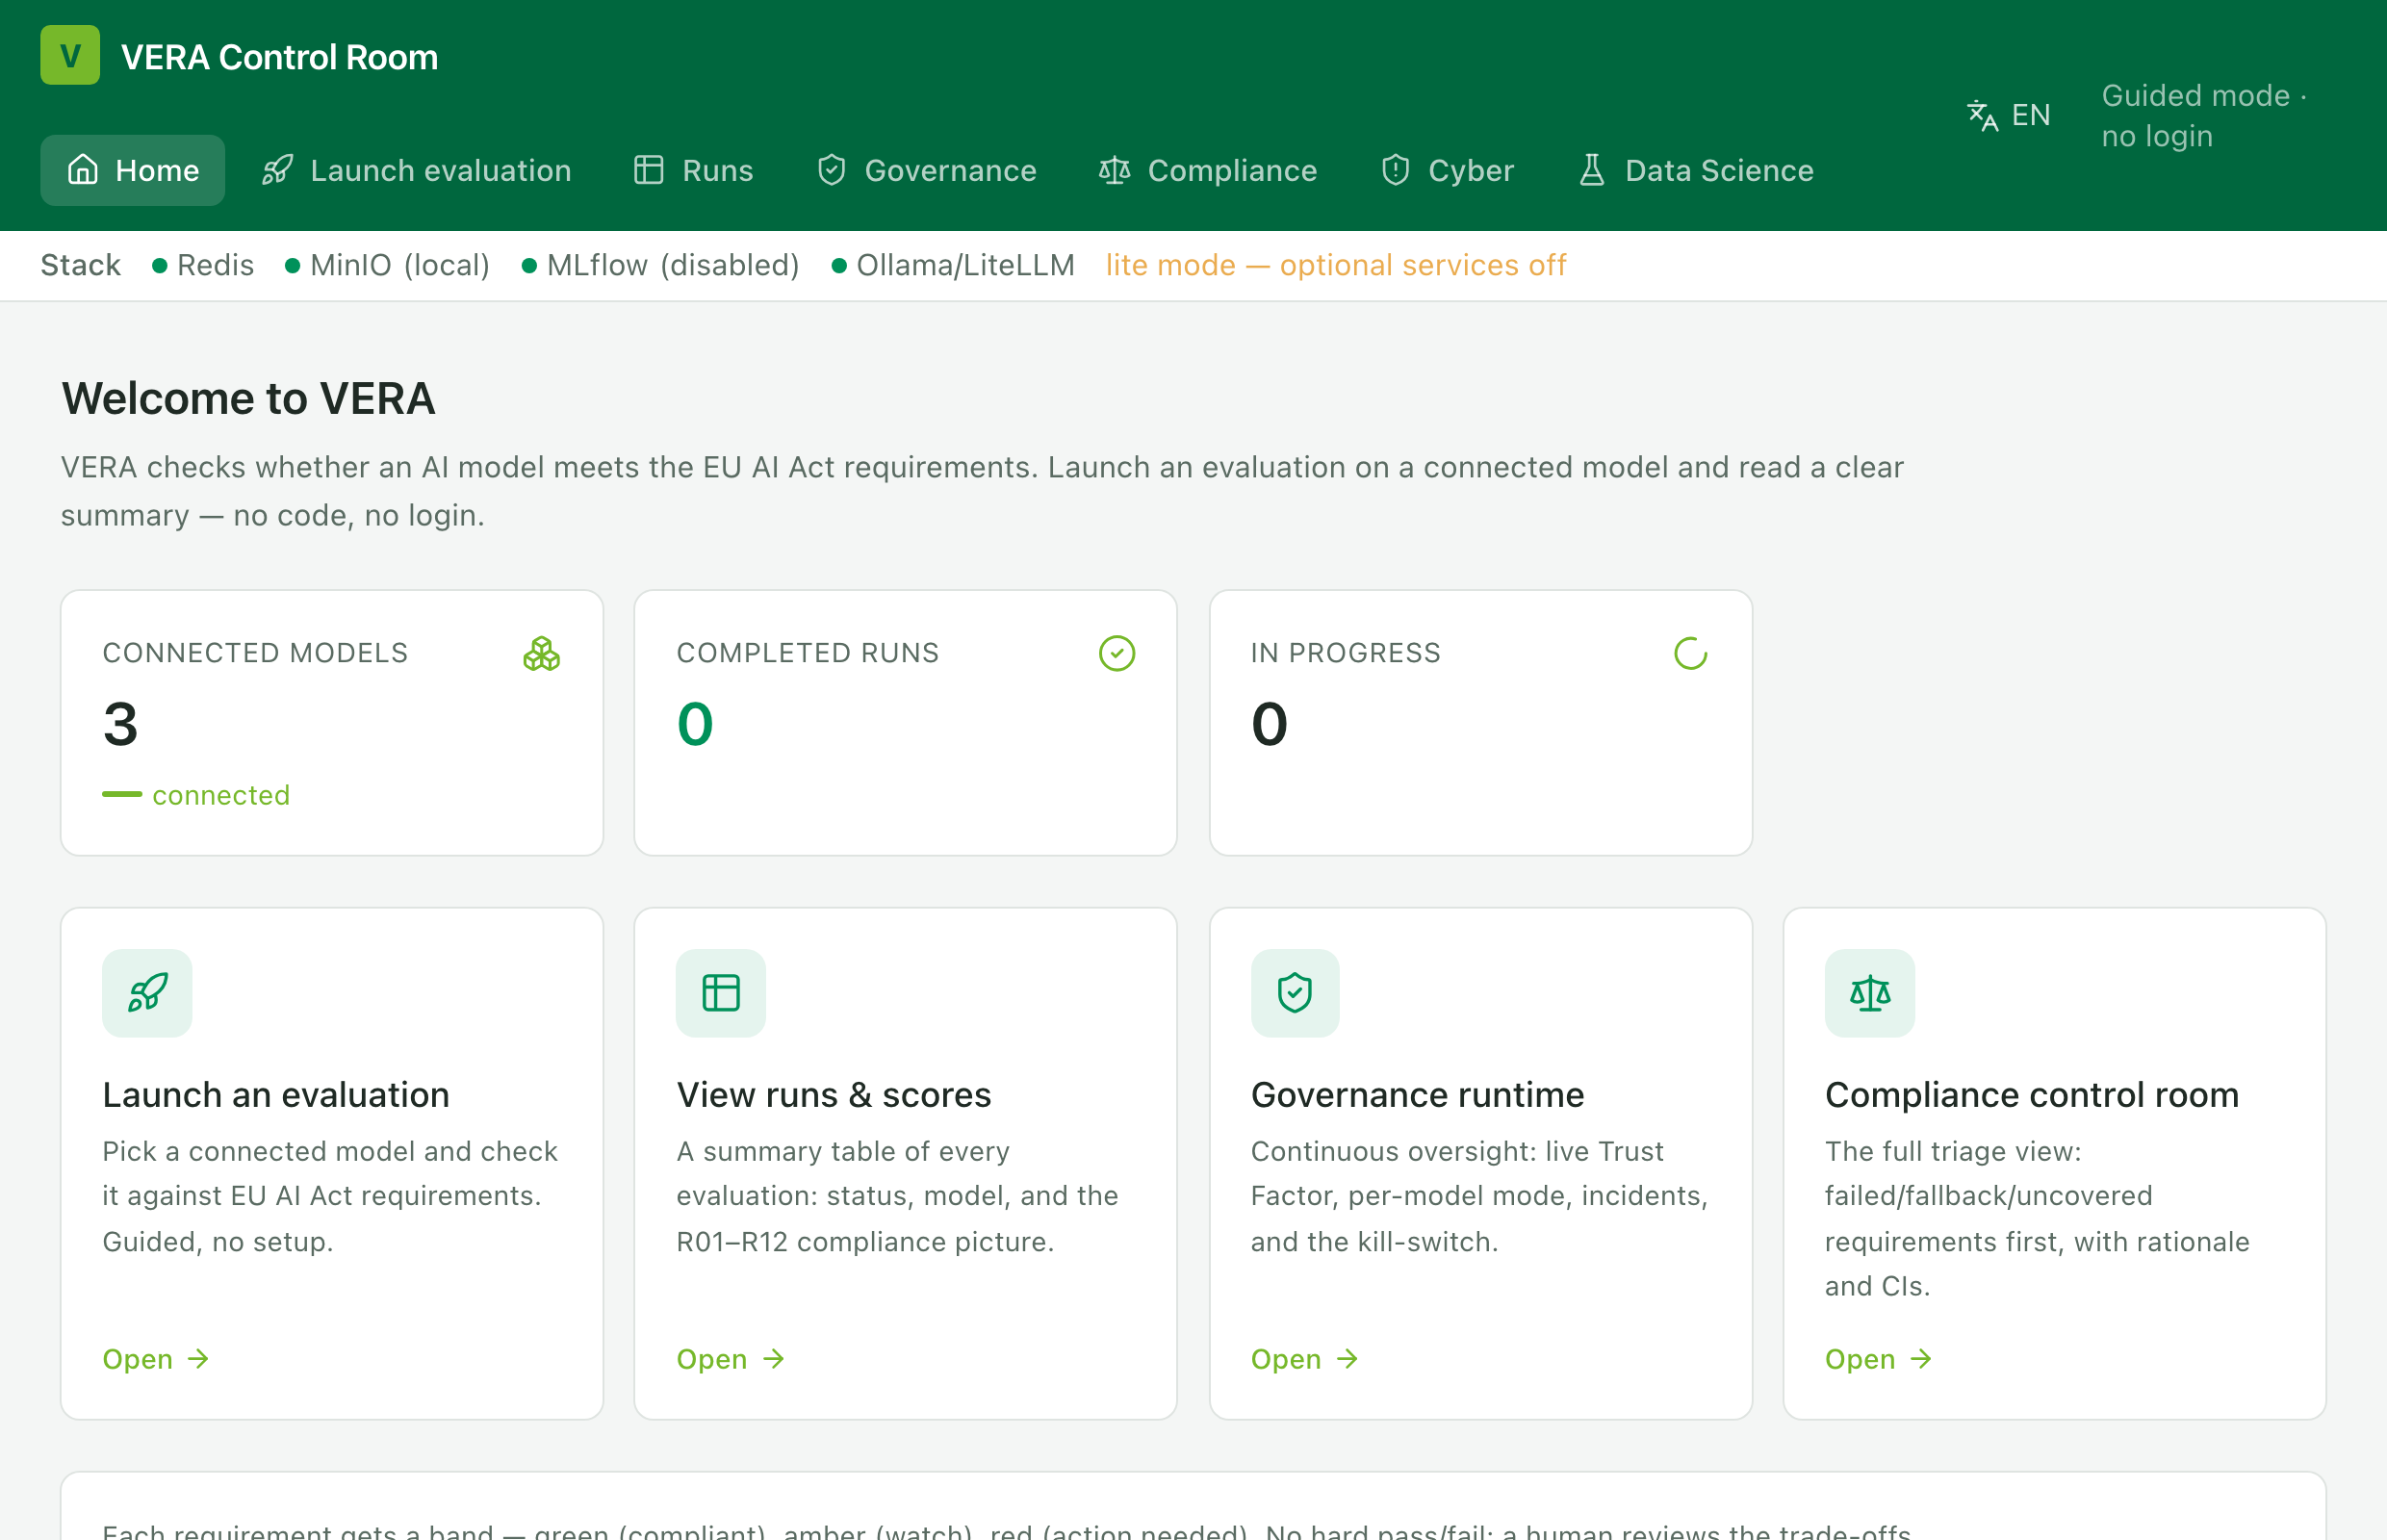
\includegraphics[width=0.86\textwidth]{figures/shot_home.png}
%   \caption{The entry point (F1, F2). A first-time visitor in guided mode sees the state of the stack, the runs already available, and a single call to action that opens the four-step launch wizard. Nothing on this page requires an account.}
%   \label{fig:home}
% \end{figure*}

% \begin{figure*}[h]
%   \centering
%   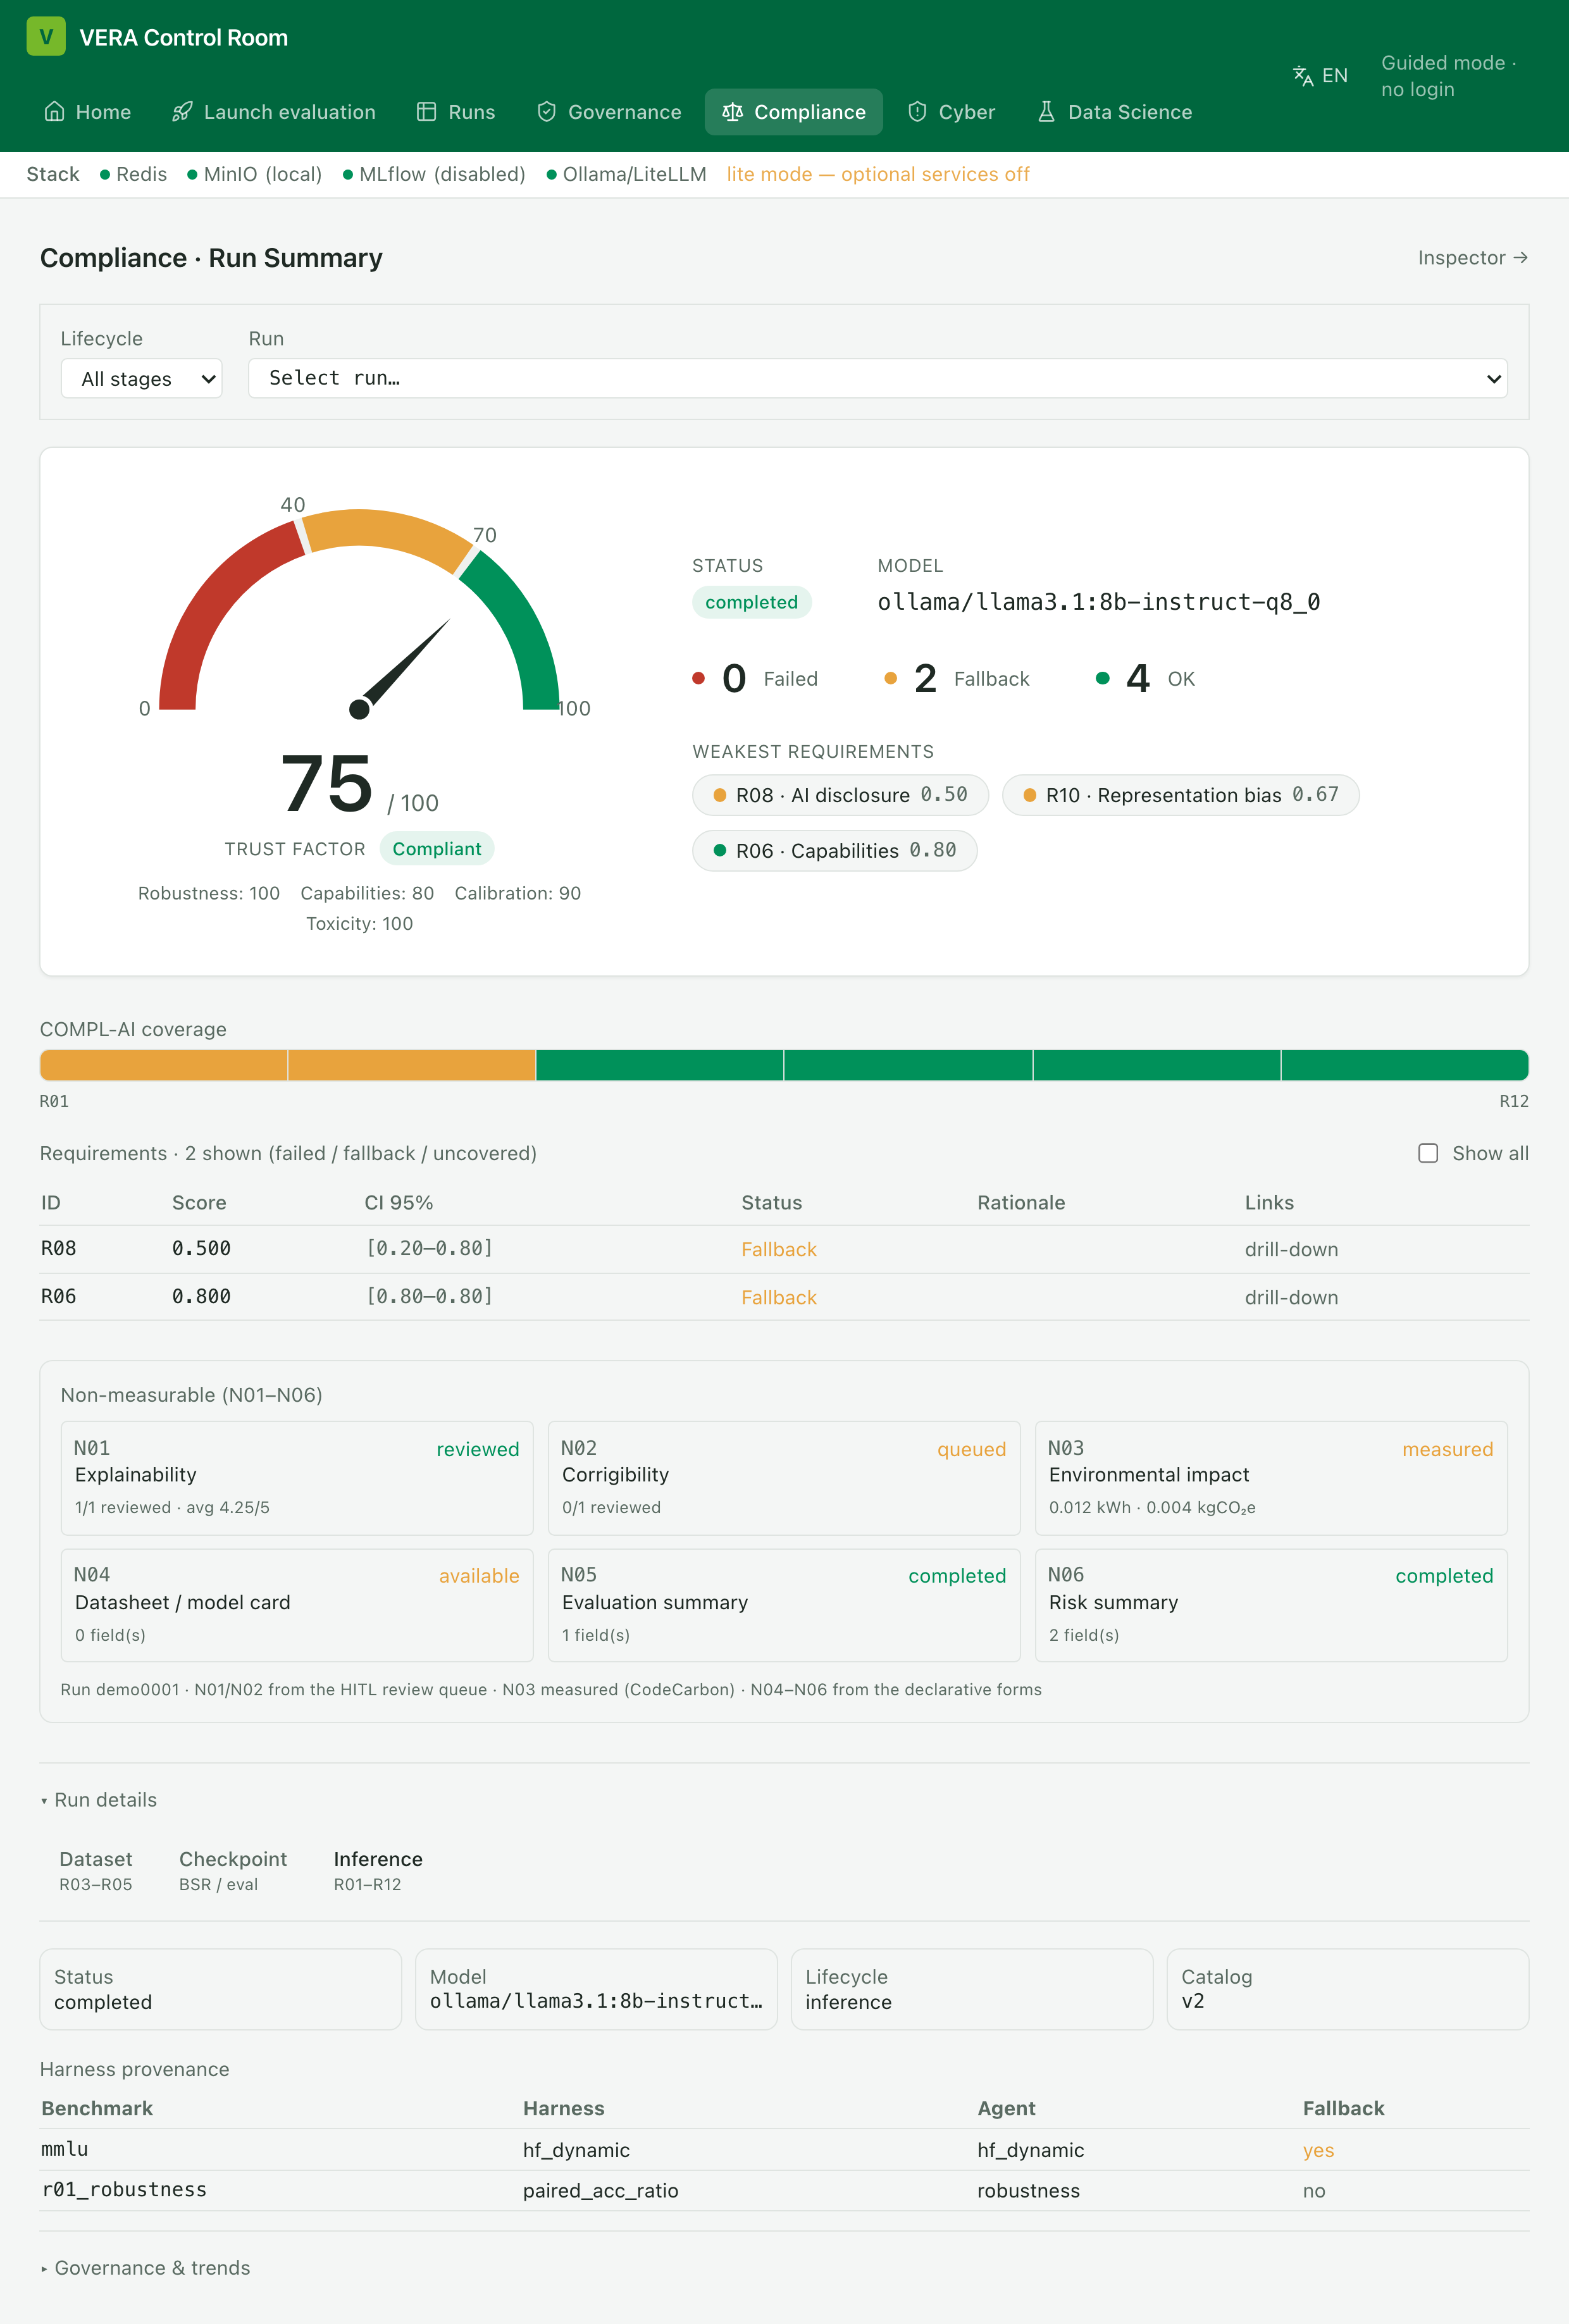
\includegraphics[width=0.72\textwidth]{figures/shot_control_room_full.png}
%   \caption{The complete run summary, of which \Cref{fig:dashboard} shows the top fold only. Below the gauge: the triage table ordered by state, the strip covering the six requirements no benchmark scores (F4), the artifacts produced by this run (F5), and the run inspector exposing the code revision, the catalog digest and the per-benchmark provenance.}
%   \label{fig:full}
% \end{figure*}

\end{document}
